\documentclass[]{msulabm}
\usepackage[utf8]{inputenc}
\usepackage{amsmath}
\usepackage{graphicx}
%\usepackage[linktocpage]{hyperref}  % if not using colorlinks, use linktocpage
\usepackage[colorlinks]{hyperref}  % if not using colorlinks, use linktocpage
\usepackage{bm}            % bold math
\usepackage{multirow}
\usepackage[table]{xcolor} % provide alternating rows with colors
\usepackage{textcomp}
\usepackage{xfrac} % gives split-level fractions with '\sfrac{a}{b}
\usepackage{multicol}
\usepackage[section]{placeins} % provides \FloatBarrier5, to keep floats from crossing this barrier
\usepackage{amssymb}
\usepackage{wrapfig} % provides wrapping figures with text.
%\usepackage{enumitem} % gives \begin{enumerate}[resume] to resume counting from previous enumerate
%\usepackage{subfigure}
%\usepackage{tikz} % to draw arrows
\usepackage{xtab} % provides xtabular, tabular environment that spans multiple pages and other awesome things
\usepackage[style=phys,biblabel=brackets,pageranges=false]{biblatex}
\usepackage{pdflscape}
\usepackage{ragged2e}
\usepackage{longtable}
\usepackage{mathabx} % gives astronomy symbols like \Earth
\usepackage{pdfpages}
\usepackage{wasysym}

\bibliography{references-manual,bbarker-zotero}

\newcommand{\abs}[1]{\left\lvert#1\right\rvert}

\title{Laboratory Manual}
\author{PHSC 12610 Black Holes \\ \\ The University of Chicago}
\date{Winter 2020}

\pagestyle{ruled}

\definecolor{lgray}{rgb}{.2,.2,.2}

\makeevenfoot{ruled}{\thepage}{\footnotesize{\textit{Last updated \today}}}{}
%\makeevenfoot{ruled}{\thepage}{}}{}
\makeoddfoot{ruled}{}{\color{lgray} \tiny{This work is licensed under \href{http://creativecommons.org/licenses/by-sa/4.0/}{CC BY-SA 4.0} by \href{mailto:bbarker@uchicago.edu}{the University of Chicago}.}}{\thepage}


% allows us to use subcaptions from the memoir class in figures. See Memoir Section 10.9
\newsubfloat{figure}

% don't worry so much about filling every page.
%\raggedbottom

% raise the penalty for splitting footnotes across different pages. Default is 100.
\interfootnotelinepenalty=10000

%\includeonly{amplifier/amplifier} 

% creates a standard length to use 
\newlength{\answerskip}
%\setlength{\answerskip}{90pt} 

%% use plus / minus if latex is squeezing the answer space too much
\setlength{\answerskip}{2cm plus 0.2cm minus 0.2cm}

\newlength{\qaskip}
\setlength{\qaskip}{\answerskip}
\addtolength{\qaskip}{\baselineskip}

% reduce vertical space between chapters in table of contents. Default is 2em.
\setlength{\cftbeforechapterskip}{1em}

% allow for extra line on a page to help prevent widow/orphan lines.
\sloppybottom

% Now we can caption a table outside of the table float environment (good for multi-page tables)
\newfixedcaption{\freetabcaption}{table}

%\includeonly{snells-law/snells-law}

\begin{document}
\maxtocdepth{chapter}

 % start roman numbering
 \frontmatter

\maketitle

%\clearpage

%Brent W. Barker

%Department of Astronomy \& Astrophysics

%The University of Chicago

%5640 South Ellis Ave.

%Chicago, IL 60637

%\href{mailto:bbarker@uchicago.edu}{bbarker@uchicago.edu}

%\vspace{2\baselineskip}

%\includegraphics{cc-by-sa-88x31}

%\textcopyright{} 2018 Brent W. Barker. Except where otherwise noted, this work is copyrighted under the Creative Commons Attribution-ShareAlike International 4.0 License. To view a copy of this license, visit \url{http://creativecommons.org/licenses/by-sa/4.0/}.

%\vspace{\baselineskip}

%These labs, excluding "Impulse and Momentum" and the appendices, are a derivative of "\href{https://%sites.google.com/site/scientificabilities/ISLE-labs}{ISLE Labs}" by the Rutgers Physics and Astronomy %Education Research group, used under the Creative Commons Attribution International 4.0 License.
%To view a copy of this license, visit \url{http://creativecommons.org/licenses/by/4.0/}.

%At Rutgers University, many people contributed to this project over the years.
%The list of names is very long and includes: Eugenia Etkina, Alan Van Heuvelen, Suzanne Brahmia, David %Brookes, Michael Gentile, Anna Karelina, Michael Lawrence, Marina Milner-Bolotin, Sahana Murthy, Maria %Ruibal-Villasenor, Aaron Warren, Xueli Zou.

 % skip to next right leaf (``recto'')
 \cleartorecto

 % the star means that the ToC itself is not listed in the ToC
 \tableofcontents*

 % start arabic numbering
\mainmatter 

\chapter{Behavior of waves (the ripple tank)}\label{cha:ripple-tank}

%TODO include theoretical limit considerations in curve fitting
%TODO for experiment 3, split setup into discrete Steps. Bold instructions to document things.

\section{Introduction}

The Michelson interferometer, named after University of Chicago professor Albert A. Michelson (Nobel prize in Physics 1907), is an extremely sensitive instrument capable of measuring incredibly tiny displacements.
A modern version of the Michelson interferometer has been developed by The Laser Interferometer Gravitational-Wave Observatory (LIGO) experiment to detect changes in distance of $10^{-19}\:$m (much less than the size of the nucleus of an atom!).
This displacement is sensed between mirrors separated by 4 km (see Figure~\ref{rt:fig:ligo-aerial}). There are two sites for LIGO --- one in Hanford, WA and the other in Livingston, LA.
The LIGO interferometer has recently detected gravitational waves for the first time (September 15, 2015); the first announced gravitational wave detection fits, with remarkable precision, the expected signal from the merging of two black holes, 29 and 36 solar masses, located 410 Mpc away.
The reported signal and the comparison to the fitted model are shown in Figure~\ref{rt:fig:ligo-signals}.

\begin{figure}
	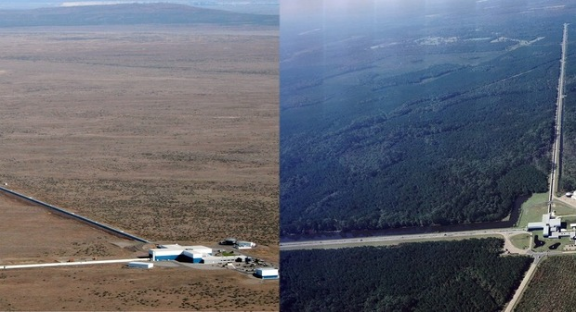
\includegraphics[width=\textwidth]{ripple-tank-remote/ligo-aerial.png}
	\caption{An aerial view of the two LIGO sites.}\label{rt:fig:ligo-aerial}
\end{figure}

\begin{figure}
	\centering
	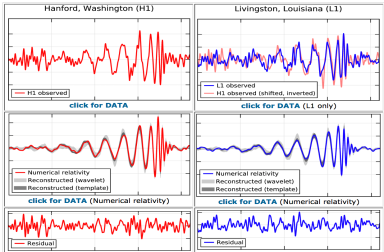
\includegraphics[width=0.7\textwidth]{ripple-tank-remote/ligo-signals.png}
	\caption{The left panels show the LIGO signal at the Hanford site (top) and the best-fit model
		(middle) and the residual of the model minus the data (bottom). The residuals are consistent
		with noise. The right panels show the same for the Livingston site, with the Hanford signal
		plotted in red in the top panel to demonstrate the similarity of the two measurements (as
		expected in the event of a true gravitational wave signal). This first LIGO detection of a
		gravitational wave event marks a significant transformation in our collective ability to
		measure and understand black holes, and since that first detection, more black hole merger
		events have been detected and reported.}\label{rt:fig:ligo-signals}
\end{figure}

The working principle of the Michelson interferometer is the interference of light.
In this lab, you will first explore the concepts of interference with sound waves, in a device known as a virtual ripple tank.
In particular, in this first portion of the lab you will experimentally discover a relationship between wave frequency and wavelength, and then demonstrate constructive and destructive wave interference.
You will then extend that understanding of interference to a wave geometry more appropriate to the second portion of the lab.
The final measurement with the ripple tank will allow you to show that plane waves propagating through a slit behave as though the slit were a new source of waves, propagating radially (i.e.\ in a circular pattern).

Next week, you will measure interference phenomena with light, with a modern version of the famous double-slit experiment performed by Thomas Young in 1801.
You will show that the interference properties of waves established in the first section of the lab apply to light as well, thus experimentally demonstrating that light behaves in a wavelike manner.

Having established the wavelike nature of light, you will then finally use a 
%table-top
virtual
Michelson interferometer to demonstrate how to measure changes in distances smaller than a human hair (not quite LIGO sensitivity, but still pretty impressive!).

\section{Learning Goals}

\begin{itemize}
	\item Learn how to conduct an observational experiment, including collecting data and analyzing the data to find and describe a pattern quantitatively.
	
	\item Discover the relationship between frequency and wavelength of waves.
	
	\item Learn how to conduct a testing experiment, including identifying a hypothesis, designing an experiment, making a prediction, and comparing it to an experimental outcome.
	
	\item Gain familiarity with wave interference.
\end{itemize}

\section{Initial planning for your project and presentation.}

Later in the course, you will write a project paper and make a presentation in lab section  on the same topic.  Project topic choices and presentation dates must be arranged with, and approved by your TA. Your choice of topic must be made in consultation with TAs and other students, so that no more than one person in any section will present on any given topic. A listing 
of ``pre-approved'' project topics is provided on Canvas. Other topics can also be accepted, with prior approval.

During the first week in lab section, \textbf{discuss the options with your TA and other students}.  By the end of your  second  lab section meeting, mutually agree on plans for your course project topic and presentation date.

%By the end of lab today, ensure that you have chosen a topic for your presentation+paper %project, and that it has been approved by your TA.

\section{Group formation}

\begin{steps}
	\item Once you have a group, meet with each other and decide a) what tools you will use to communicate and collaborate, b) when you will meet, c) what you will do when you need to change an agreement, and d) what you will do when a member has a concern about how the group is functioning. \textbf{Record your agreements in your lab report.} %This part counts as data collection and analysis, so it can be identical in each member's report.}
\end{steps}

\subsection{Team roles}

\begin{steps}
	\item \textbf{Decide on roles} for each group member.
\end{steps}

The available roles are:

\begin{itemize}
	\item Facilitator: ensures time and group focus are efficiently used
	\item Scribe: ensures work is recorded
	\item Technician: oversees apparatus assembly, usage
	\item Skeptic: ensures group is questioning itself
\end{itemize}

These roles can rotate each lab, and you will report at the end of the lab report on how it went for each role. If you have fewer than 4 people in your group, then some members will be holding more than one role. For example, you could have the skeptic double with another role. Consider taking on a role you are less comfortable with, to gain experience and more comfort in that role.

Additionally, if you are finding the lab roles more restrictive than helpful, you can decide to co-hold some or all roles, or think of them more like functions that every team needs to carry out, and then reflecting on how the team executed each function.

\subsection{Add members to Canvas lab report assignment group}

\begin{steps}
	\item On Canvas, navigate to the People section, then to the ``Lab 1 Groups'' tab. Find a group that is not yet used, and have each person in your group add themselves to that same lab group.
\end{steps}

This enables group grading of your lab report. Only one person will submit the group report, and all members of the group will receive the grade and have access to view the graded assignment.

\section{The Scientific Cycle\protect\footnote{adapted from \cite{etkina_college_2014}}}

One way of describing science is the process of incrementally improving a shared model of how our universe works. In different fields of science, different methods and cycles are used, so there is no ``One True Scientific Method.'' One can still create a model for the process of science, and we describe here one such cycle (the hypothetico-deductive cycle), summarized in Figure~\ref{me:fig:isle}.

In this cycle, there are three types of experiments, each one representing a different stage of the scientific effort. One stage, often started when encountering a novel phenomenon, is the \textbf{observational experiment}. This is an experiment that consists of deciding what to observe and how to observe it, collecting data, finding a pattern, and brainstorming possible explanations for what is observed (also called ``hypotheses'').

Once one has some trial explanations, one can test one or more of those with a \textbf{testing experiment}. Here, one designs a new experimental procedure and uses each hypothesis to predict what will happen. Then the prediction is compared to the procedure's outcome. If they are different, then the hypothesis is judged to be not a helpful explanation for that phenomenon. If they are the same, then it is still helpful. Throughout this stage, one may make various assumptions that would need to be validated, as they can effect the prediction or outcome.

Once a hypothesis has been tested enough for people to find it useful, then it can be applied to solve practical problems, or to determine properties of particular situations, in an ``application experiment.''

\begin{figure}
	\centering
	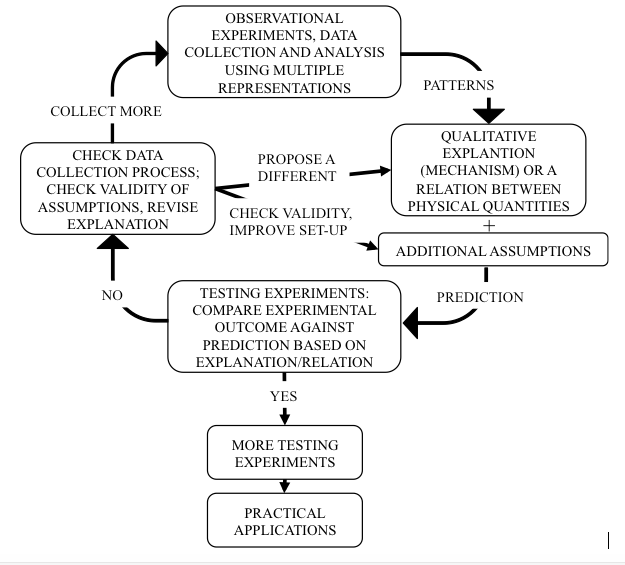
\includegraphics[width=0.7\textwidth]{ripple-tank-remote/islegraphic.png}
	\caption{A model of the process some scientists go through to create knowledge.\cite{etkina_millikan_2015}}\label{me:fig:isle}
\end{figure}

\section{Experiment 1: Observation of frequency and wavelength}

\subsection{Goal}

Observe sound waves in a virtual ripple tank and determine a mathematical relationship between frequency and wavelength.

\subsection{Available equipment}

\begin{itemize}
	\item virtual ripple tank at \url{www.falstad.com/ripple}
\end{itemize}

%ripple tank with strobe light and ripple generator, plane wave attachment, 2 dippers (narrow plastic rods), 1 short wall, 1 medium wall, 2 long walls for ripple tank, flashlights or desk lamps, digital camera (e.g.\ your smartphone), computer with ImageJ installed (can be your device), object of known size to be submerged

%\begin{framed}
%	\textbf{Caution: Flickering Lights!} You will be using a stroboscopic light in this lab. Such light is known to trigger reactions in some individuals (e.g. photosensitive epilepsy).
%	If you are worried that you may be sensitive to strobe light, speak to the TA and skip attending this part of the lab.
%	In any case, avoid staring directly at the light.
%\end{framed}

\begin{framed}
	\textbf{Self-assessment:} To help you improve your scientific abilities, we provide you with self-assessment rubrics.
	A rubric is a scoring system.
	Self-assessment is determining how well you performed a particular task.
	So, these self-assessment rubrics are designed to help you evaluate your performance while you are designing and performing your experiment.
	
	The complete set of rubrics is available in Appendix~\ref{cha:rubrics}.
	In each lab, your report will be assessed using Rubric F, found in Table~\ref{rubric:f}, as well as 5 additional rubric rows listed in that lab.
	Each week, read through these and use them to evaluate your work as you design and perform the experiment.
	Your instructor will use the same rubrics to determine part of your grade for the lab.
\end{framed}	

\subsection{Rubrics to focus on during this experiment}

B7, B8, F1, F2. See Appendix~\ref{cha:rubrics} for details.

\subsection{The virtual ripple tank}

\begin{steps}
	\item Open the virtual ripple tank by going to \url{www.falstad.com/ripple} in a web browser.
\end{steps}

This is a simulation that demonstrates waves in two dimensions. The waves can represent water waves, sound, and light. When the simulation starts up, you will see a white square (called the ``source'') emitting circular waves. The light areas are positive and the dark areas are negative. So, if you prefer to think of the waves as sound waves, the light areas would be areas of high pressure, and the dark areas would be low pressure. The source might be a speaker of some sort. You can drag the source around wherever you want. Also you can create new waves (areas of high pressure) by clicking anywhere.

As you move the pointer around the tank, the position coordinates of the pointer, as well as the current time in the simulation, are displayed in the lower left corner.  Note that the simulation is showing a slowed-down version of the actual sound waves, so the time in the simulation will pass much slower than the actual time.

The sliders to the right of the tank control various aspects of the simulation. For the frequency slider in particular, if the waves are set to represent sound, then the frequency of the emitted sound is equal to the number to the right of the slider times 54, with units of hertz (Hz, or cycles per second).

%In this section you will explore interference phenomena using a ripple tank. The tank --- 42.5 cm x 42.5 cm and 2.5
%cm deep --- is filled with water, and is equipped with a ripple generator. The generator uses voice coil actuators to
%produce the precise and quiet up-and-down motion of the rippler arms. Waves are generated in the tank by the moving
%dippers that touch the surface of the water. The generator also controls a light source that produces a bright, clear
%image of the wave patterns in the ripple tank. The light can be used as a steady source or as a strobe to ‘freeze’ the
%motion of the wave patterns (in this case the flashing light and the generator are driven with the same frequency). The
%ripple generator frequency ranges from 1.0 to 50 Hz adjustable in 0.1 Hz increments. You will work with frequencies in
%the range 16--32 Hz. A mirror placed below the tank and working in conjunction with a projection screen provide a
%magnified image of the wave patterns in the water; you will record patterns seen on this screen by photographing them
%with a digital camera. The ripple generator terminates in a bar with numerous clips in which you can place various
%``dippers''.

\subsection{Suggestions for your experiment}

\begin{steps}
%	\item You may want to decide on roles for each group member. Example roles include Facilitator (ensures time and group focus are efficiently used), Scribe (ensures work is recorded), Technician (oversees apparatus assembly, usage), Skeptic (ensures group is questioning itself). Note that each role is responsible for ensuring that the thing happens, rather than necessarily doing it themselves. \textbf{Decide if you are using these roles, and if so, assign them and note them in the lab report.}
	
	\item Ensure that every group member knows what the terms frequency and wavelength mean, in relation to waves. Use whatever means at your disposal to do this.
	
	\item This is an ``observational experiment.'' Review Rubric B (Table~\ref{rubric:b}) and discuss any unclear expectations with your group and the instructor. Note that your lab report will be graded, in part, on demonstration of Abilities B7 and B8.
	
%	\item Ensure that one of the ripple tank's ripple generator is set up with 1 dipper fixed in the center clip of the bar that extends from the box, and that the height of the generator is such that the dipper just touches the top of the water. You can make coarse adjustments by moving the generator along the support rod, and fine adjustments with the two red knobs on it.
	
	\item Brainstorm different methods you could use to determine the relationship between wavelength and frequency. Feel free to play with the simulation as you do so, seeing what the various sliders and checkboxes on the right do. Here are some things to consider:
	\begin{itemize}
		\item Which variable will you control (and thus will be the independent variable) and which will you measure?
		
		\item What is the range of the independent variable that you will use? How many different settings will you choose?
		
		\item You will need to use several settings of the independent variable, and then plot the data in a graph, decide on what pattern you see, and give some justification for that pattern. You can use words like ``proportional'', ``linear'', ``parabolic'', ``exponential'', ``logarithmic'', and so on, if they fit. Ensure you use the mathematical definition of these.
		
		\item How will you measure the wavelength? Is it a more precise measurement if you measure several of them at once and divide to get a single wavelength? You can use these coordinates to calculate the distance $d$ between two points on the screen, $(x_1, y_1)$ and $(x_2, y_2)$, using the Pythagorean theorem
		\begin{equation}
		d = \sqrt{(x_2-x_1)^2+(y_2-y_1)^2} \,.
		\end{equation}
			
%			\item The reflected image might magnify the ripple tank, so it can be helpful to place an object of known size in the tank, like a coin, so you can determine the correct scaling.
%		\end{itemize}
		
%		One way to take careful measurements of the wavelength is to take a picture of the projected tank, then use a program like ImageJ to measure the lengths you need. If you do so, one way to keep track of what settings go with what image is to mark a card with the settings and place it in view of the camera. See the section below on measuring lengths with ImageJ.
	\end{itemize}

	\item Decide on your measurement and analysis method and discuss it with an instructor before you begin. They will help increase the chances that your method will lead to successful results, or at least that the unhelpful path that you choose will take a short enough amount of time for you to change it when you discover it does not work. We want you to have productive failure that you have time to learn from.
	
	\item Perform your experiment. Your lab report for this experiment should include:
	\begin{itemize}
		\item A labeled sketch or photo of the setup, and a description of the experimental procedure (see Rubric F1).
		
		\item A plot of wavelength vs. frequency (with the independent variable on the horizontal axis)
		
		\item A description of the pattern found. This can be done with a line (straight or curved) showing the pattern you see (either drawn manually or using the curve fitting function of the plotting program, e.g.\ LibreOffice Calc or Microsoft Excel) and with words describing what you found. (B7)
		
		\item An equation to represent the pattern. This can be taken from a curve fit or found by hand. Make sure there is some discussion of how well the equation agrees with the data, but you don't need to be very precise about it. (B8)
		
		\item A discussion of the findings of the experiment and why it's helpful (for you and/or for science) (F2)
	\end{itemize}

\end{steps}

%\subsection{Measuring lengths using ImageJ}
%
%ImageJ (\url{http://imagej.nih.gov/ij/download.html}), which is installed on the lab computers, is useful for measuring lengths in images. To do so, load your image, then follow these steps to calibrate the ruler --- that is, to tell ImageJ how long something is in the image, so it knows how many pixels correspond to what length).
%
%\begin{enumerate}
%	\item Start with an image that has an object in it that you know one of the lengths of (e.g.\ the length of side, or a diameter).
%	
%	\item Open that image in ImageJ.
%	
%	\item Select the icon with the straight line on it, and click and drag along the known length.
%	
%	\item From the drop-down menu, select ``Analyze'' $>$ ``Set Scale...''.
%	
%	\item Set ``Known distance'' to the value of the known length.
%	
%	\item Set ``Unit of length'' to the unit you are using, for example ``mm'' for millimeters.
%	
%	\item Record the pixel scale given at the bottom of the box for future use.
%	
%	\item Now when you use the straight line tool, it will give the length in physical units in ImageJ's toolbar.
%\end{enumerate}

\section{Experiment 2: Testing the conditions for destructive interference}

\subsection{Goal}

A student from a different lab section came up with the idea that destructive interference between two waves occurs at positions where the distance from each source differs by an integer number of wavelengths, or
\begin{equation}
 \Delta d = m\lambda \,,
\end{equation}
where $\Delta d$ is the ``path length difference'', $\lambda$ is the wavelength, and $m$ is any integer. The student has asked you to test this idea for them. Please do so and provide them feedback.

\subsection{Available equipment}

\begin{itemize}
	\item Same as in the previous experiment
\end{itemize}

\subsection{Setup}

From the ``Example'' drop-down menu on the right, select ``Example: Two Sources''.
%1 dipper, use two dippers mounted with 3 empty clips between them on the bar. Ask the TA for assistance in setting this up. Adjust so that the dippers are just resting in the surface of the water. Adjust the frequency and amplitude to get clear, sharp waves.

\subsection{Rubric rows to be assessed in this experiment}

C1, C4, C7, F1, F2. See Appendix~\ref{cha:rubrics} for details.

\subsection{Testing this hypothesis}

In general, one tests a hypothesis by using it to make a prediction about what will happen in a certain experimental procedure. With this hypothesis, it asserts a relationship between path length difference, wavelength, and destructive interference.

Destructive interference occurs whenever two waves overlap and attempt to disturb the medium in opposite directions, resulting in no disturbance. In this case, the color is the original color of the tank, neither lighter nor darker. In the 3-D view, the places of destructive interference are where the surface does not move up or down during the wave motion.

%But there are only certain points on the ripple tank image where it is easy to see constructive interference --- the bright spots at the intersection of waves originating from both sources. For an example, see Figure~\ref{rt:fig:interference-2d}.

%\begin{figure}
%	\centering
%	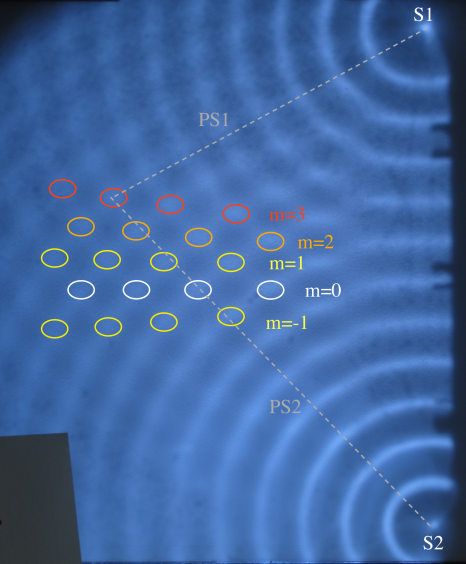
\includegraphics[width=0.7\textwidth]{ripple-tank-remote/interference-2d.png}
%	\caption{Example interference pattern for 2 dippers. The bright spots are circled. For a particular bright spot of constructive interference, the two path lengths PS1 and PS2 are drawn.}\label{rt:fig:interference-2d}
%\end{figure}

In this case, it is easier to start by finding those locations, picking a particular point, measuring the $\Delta d$, finding the wavelength for the given frequency using the relationship you found in Experiment 1, and solving for $m$. The hypothesis predicts that $m$ should always be an integer. As a result, your experiment becomes this: find out how close the experimentally determined $m$'s are to integers.

Brainstorm your experimental procedure, decide on it, discuss with your TA, then perform the experiment.

Your lab report for this experiment should include:
\begin{itemize}
	\item A clear description of the hypothesis (see Rubric C1).
	
	\item A labeled sketch or photo of the setup, and a description of the experimental procedure (F1).
	
	\item A clear statement of the prediction that the hypothesis makes for this particular procedure (C4).

	\item A table of path lengths, path length differences, and measured $m$ values.
	
	\item An analysis of how close the measured $m$ values are to the prediction. Use some quantitative measure of this, but don't worry about being precise about uncertainties (C7).
	
	\item A judgment about the hypothesis. Is it supported, disproved, or undetermined? (C8, though not assessed this time)
	
	\item A discussion of the findings of the experiment and why it's helpful (for you and/or for science) (F2).
\end{itemize}

\section{Group functioning}

\begin{steps}
	\item Write a 100--200 word reflection on group dynamics. Address the following topics: who did what in the lab, how did you work together, how group roles functioned, what successes and challenges in group functioning did you have, and what might you want to do differently next time?
\end{steps}

%In the case of a hypothesis like this one, that includes a proposed equation, there is a useful template for coming up with a prediction:
%\begin{enumerate}
%	\item Note that this hypothesis is asserting that when the equation is true, there is constructive interference (a bright spot). So the goal is to test how true this is.
%	
%	\item Choose which variables you are holding constant, which one is the independent, and which is the dependent variable. In this case, you may not know what $m$ is ahead of time. You could choose it arbitrarily, for example $m=0$ first, and go from there.
%	
%	\item Once you decide on your procedure (which things to measure, how to vary the independent variable), you can use the equation to solve for the dependent variable, which becomes the prediction (Rubric C4).
%	
%	\item The set of dependent variables (for each chosen independent variable) becomes the prediction of the hypothesis that you will use to compare to experimental outcome (C7).
%\end{enumerate}
%
%\subsection{Suggestions for your experiment}
%
%\begin{itemize}
%	\item Note that constructive interference happens where there are bright spots in the projected image at the intersection of waves coming from both sources.
%	
%	\item There is an entire line of points that have the same path length difference from each source, so for each choice of $m$, there can be many 
%\end{itemize}

\section{Individual Homework: Observing plane waves encountering narrow gaps}

These questions are to be answered individually and your answers should be submitted under the Lab 1 Homework assignment on Canvas.

This experiment does not clearly follow the model of the scientific cycle, but is closest to an observational experiment. In next week's lab, you will investigate the properties of light traveling through small slits. Ripples in a virtual tank are more obviously waves, so it is helpful to observe what happens here first.

\begin{enumerate}
	\item Instead of point sources, select the ``Example: Single Slit'' and then set ``Waves = Sound''. This example is of a straight line wave, or, in two dimensions, a ``plane wave'', incident on a wall with a small opening. This is the same kind of wave and apparatus we will use next week with light. What wave pattern do you see? How does this pattern compare to the data you took using one source?
	
	\item Is the wavelength of the pattern you observe consistent with the relationship between frequency and wavelength you
	measured with single point source? Include any measurements and calculations you make in answering this question in your homework response, and be quantitative.
	
	\item Select ``Example: Double Slit'' and then set ``Waves = Sound''. What wave pattern do you see? How does this pattern compare to the data you took using two sources?
	
\end{enumerate}
	


	

	
%Adjust the amplitude and frequency, with the frequency in the range 20--25 Hz, until you see
%clear well-defined vertical parallel lines. Now, insert the two large ``walls'' in the tank, parallel to the rippler bar and
%perhaps 5cm away; allow a small (few mm) opening between the two wall sections, placed so that opening is vertically
%centered in the projected image. Adjust the amplitude upward until you see a clear wave pattern radiating from that
%opening. Take a picture. Repeat this with two apertures instead of one; do this by adding a smaller wall between the
%two larger sections, with all sections parallel to the rippler bar, and a small gap between each larger wall and the central
%smaller portion. Again, take a picture, adjusting amplitude as necessary to get well-defined waves.
%
%The analysis of this will be done as individual homework.
%
%\section{Individual Homework}
%
%These questions are to be answered individually and your answers should be submitted under the Lab 1 Homework assignment on Canvas.
%
%Both questions concern the last two situations recorded in the lab: the case of 2 walls (1 gap or ``aperture'') and the case with 3 walls (2 apertures).
%
%\begin{enumerate}
%	\item What wave pattern do you see in the case of a single slit? What do you see in the case of a double slit?
%	How do these patterns compare to the data you took using one and two sources?
%	
%	\item Is the wavelength of the pattern you observe consistent with the relationship between frequency and wavelength you
%	measured with the point sources? Include any measurements and calculations you make in answering this question in your homework response, and be quantitative.
%\end{enumerate}
\chapter{Behavior of electromagnetic waves in space (lasers and slits)}

\section{Introduction}

In 1801, Thomas Young's ``double-slit'' experiment demonstrated the wave nature of light by showing that two coherent light sources produce interference patterns. You will perform a modern version of Young's experiment using a
laser as light source. The laser illuminates two thin slits, each of width $a$ separated by a distance $d$, which act as two
coherent sources of light. This is analogous to what you have observed with water waves in the previous lab section, in
which you saw a plane wave combined with an aperture (a slit) acting as a circular source of waves. An interference
pattern appears on a viewing screen, placed at a distance $L$ from the double slit, in the form of bright and dark regions
corresponding to maxima and minima of interference. You will use the interference pattern to measure the wavelength
$\lambda$ of the laser, and show that the same framework of equations that is derived in the introduction to the previous lab
holds for light too.

\section{Topic selection for individual paper and presentation}

By the end of lab today, ensure that you have chosen a topic for your individual project, and that it has been approved by your TA.

\section{Team roles}

\begin{steps}
	\item \textbf{Decide on roles} for each group member.
\end{steps}

The available roles are:

\begin{itemize}
	\item Facilitator: ensures time and group focus are efficiently used
	\item Scribe: ensures work is recorded
	\item Technician: oversees apparatus assembly, usage
	\item Skeptic: ensures group is questioning itself
\end{itemize}

These roles can rotate each lab, and you will report at the end of the lab report on how it went for each role. If you have fewer than 4 people in your group, then some members will be holding more than one role. For example, you could have the skeptic double with another role. Consider taking on a role you are less comfortable with, to gain experience and more comfort in that role.

Additionally, if you are finding the lab roles more restrictive than helpful, you can decide to co-hold some or all roles, or think of them more like functions that every team needs to carry out, and then reflecting on how the team executed each function.

\section{Add members to Canvas lab report assignment group}

\begin{steps}
	\item On Canvas, navigate to the People section, then to the ``Lab 2 Groups'' tab. Find a group that is not yet used, and have each person in your group add themselves to that same lab group.
\end{steps}

This enables group grading of your lab report. Only one person will submit the group report, and all members of the group will receive the grade and have access to view the graded assignment.

\section{Experiment 1: Observing patterns made by 1 and by 2 slits}\label{li:sec:exp1}

\subsection{Goal}

Describe the patterns made by a laser that is incident on 1 slit and on 2 slits, and the differences and similarities between them.

\subsection{Available equipment}

\begin{itemize}
	\item In this remote environment, imagine you have a laser, slit card, and screen as shown in Figure\ \ref{lir:fig:setup}.
\end{itemize}

\begin{figure}
	\centering
	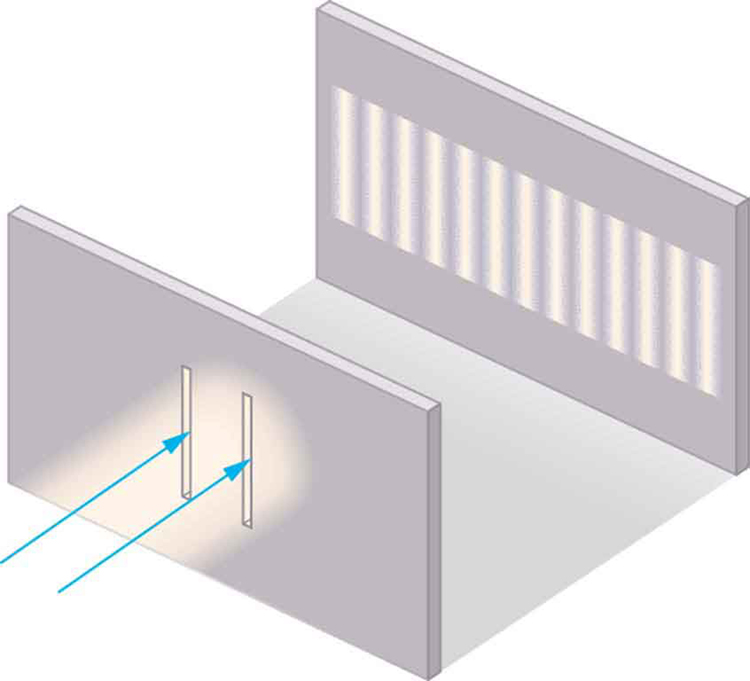
\includegraphics[width=0.5\textwidth]{laser-interference-remote/double-slit-setup.jpeg}
	\caption{Setup for the double-slit experiment. Laser light of a single frequency is sent through
		two slits and a pattern forms on the screen. Figure from OpenStax. Access for free at \url{https://openstax.org/books/college-physics/pages/27-3-youngs-double-slit-experiment}}\label{lir:fig:setup}
\end{figure}

\begin{figure}
	\centering
	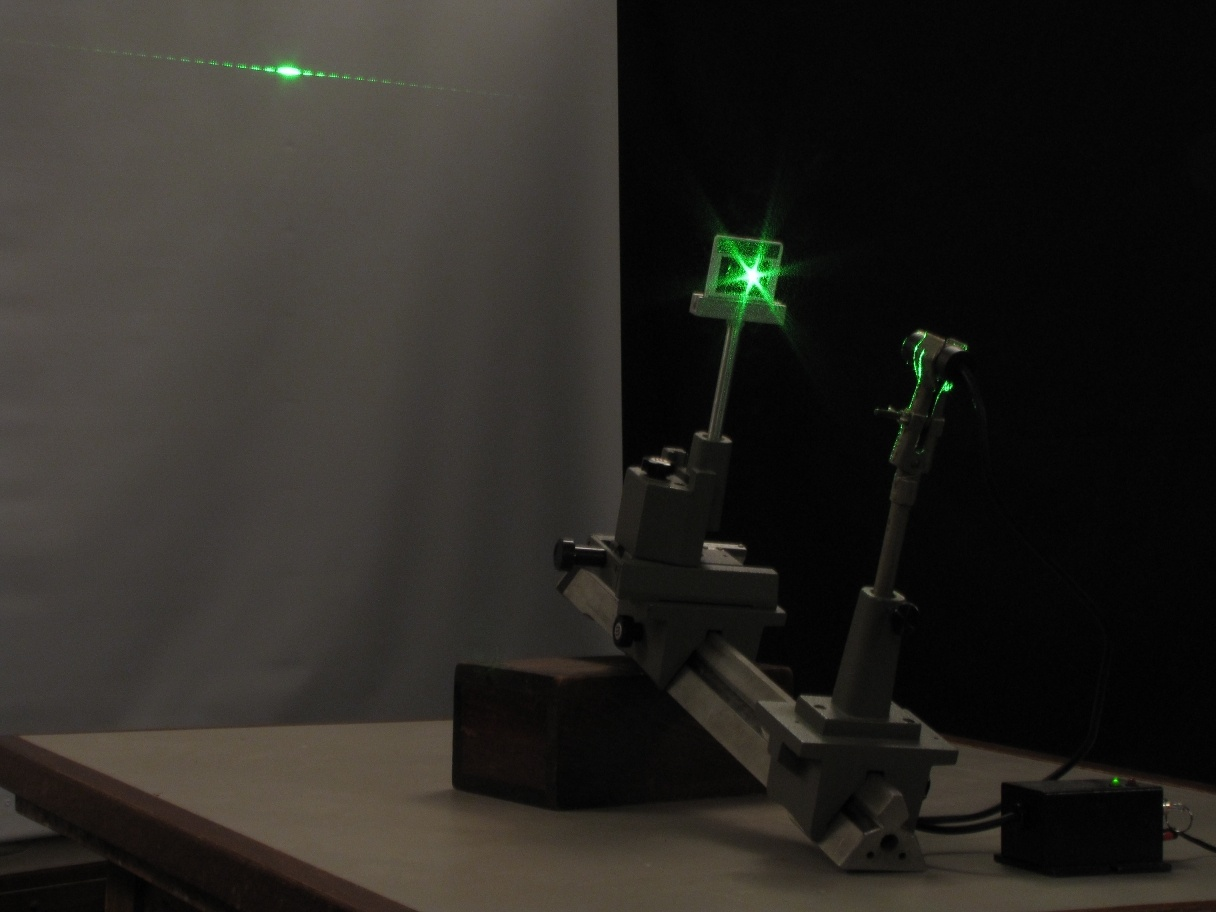
\includegraphics[width=0.5\textwidth]{laser-interference-remote/laser_double_slit_intererfence.JPG}
	\caption{Setup for the double-slit experiment. Laser light of a single frequency originates from the laser on the right. The laser light strikes the card in the middle, some of it passing through two thin vertical slits. A pattern forms on the screen. Image from \url{https://wiki.uchicago.edu/display/KER/Laser+Double+Slit+Interference} }\label{lir:fig:setup-photo}
\end{figure}

%optical bench, viewing screen, blank white paper, PASCO ``Multiple Slits'' assembly, red laser with mounting clamp, support stand, optionally computer with ImageJ installed

%\begin{framed}
%	\textbf{Warning: Laser Hazard!} The power of our lasers is low enough that the normal human blink reflex is sufficient to protect against incidental eye exposure.
%	
%	That being said, the following rules reduce the risk of eye exposure to laser light:
%	\begin{enumerate}
%		\item Do not direct the laser beam into anyone's eye.
%		\item Be aware of the laser reflecting off of mirror-like surfaces and where that beam goes.
%		\item Turn off the laser when not in use.
%		\item Keep the laser pointing horizontally and near the plane of the table, while keep your eyes above that plane.
%		\item To determine whether the laser is on, put your hand or a light-colored object in front of the beam, rather than looking into the laser aperture.
%	\end{enumerate}
%\end{framed}

\subsection{Rubrics to be assessed for this section}

F1, F2. See Appendix~\ref{cha:rubrics} for details.



%\subsection{Setup}
%Ensure the red laser is turned on and pointed at the slit assembly. Rotate the head of the slit assembly so that the active slit is the ''Comparison'' slit location with both a single
%and double slit furthest counter-clockwise. Adjust the laser so that the active slit
%is well illuminated by the laser spot. Note the laser should be pointed slightly upward if the laser head is ~10cm off the
%table, and pointed so it hits the screen ~5cm from the top edge, and so moving the slit assembly closer to the laser will
%move the spot on the slit assembly lower, and moving it further will move the spot higher. With the slits aligned with the
%laser, you will see light on the screen, but no longer a simple spot. Instead, you will see a vertical feature, the details of
%which depend on whether the laser is illuminating the single slit, or the double slit. Nudge the rail end back and forth to
%see the difference.

\subsection{Steps}

In our lab of the mind, we have a red laser sending a thin beam of light of a single wavelength through slits and onto a screen. A sketch of the situation is shown in Figure\ \ref{lir:fig:setup}, and a photo of the setup is shown in Figure\ \ref{lir:fig:setup-photo}. We first use just a single slit, and then use both of them. With the room lights off, we take a picture of each case. The results are shown in Figure\ \ref{lir:fig:patterns}.

\begin{figure}
	\centering
	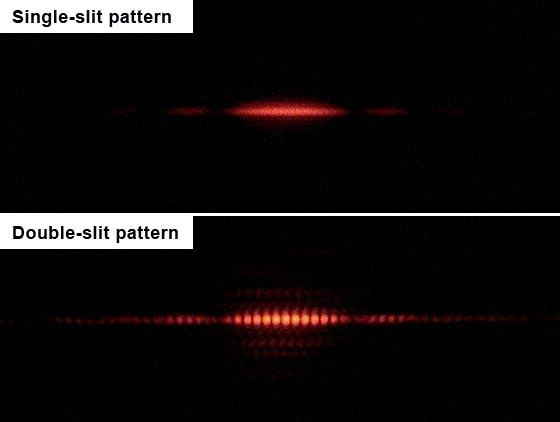
\includegraphics[width=0.6\textwidth]{laser-interference-remote/Single_slit_and_double_slit2.jpg}
	\caption{In a dark room, a laser is aimed at a card with a single or double slit in it. The light passes through the slit(s) and lights up a screen with the patterns shown. Image from \url{https://en.wikipedia.org/wiki/Double-slit_experiment\#/media/File:Single_slit_and_double_slit2.jpg}}\label{lir:fig:patterns}
\end{figure}

\begin{steps}
	\item Discuss the patterns observed in Figure\ \ref{lir:fig:patterns}. Describe each in detail. How are they alike and different? \textbf{Record your description and comparison.}
\end{steps}

\section{Experiment 2: Testing the wave hypothesis}\label{lir:sec:exp2}

\subsection{Goal}

Determine whether light from a laser can be described as a plane wave.

\subsection{Available equipment}

%Same as in Section~\ref{li:sec:exp1}, plus a green laser with mounting clamp

\begin{itemize}
	\item Simulation of laser light passing through slits, found at \url{https://physics.bu.edu/~duffy/HTML5/double_slit.html}
\end{itemize}

\subsection{Rubrics to be assessed for this section}

C4, C7, C8, G2, G4, F1, F2. See Appendix~\ref{cha:rubrics} for details.

\subsection{Behavior of a plane wave incident on single and double slits}

The following equation describes the location, $y_m$ (measured relative to the center of the pattern), of the $m$th interference \textit{minimum} (dark spot) seen on a screen when a plane wave is incident on a single slit.
\begin{equation}
y_m = \frac{m \lambda L}{a} \,,
\end{equation}
where $L$ is the distance from the slit to the screen, and $a$ is the width of the slit.

For a double slit, the following equation describes the location $y_n$ of the $n$th interference \textit{maximum} (bright spot) seen on a screen when a plane wave is incident on a double slit.
\begin{equation}
y_n = \frac{n \lambda L}{d} \,,
\end{equation}
where $d$ is the distance between the two slits. These equations use the same principle of path length difference as used in the previous lab, but are derived for the case where the distance from slit to screen is much larger than the slit and spacing dimensions.

\subsection{Suggestions for your experiment}

\begin{itemize}
	
%	\item \textbf{REQUIRED:} Use both the green laser and the red laser for this experiment, and ensure that you keep the data (image and setup parameters) for use in the individual homework.
	
%	\item For measuring the interference minima and maxima, you can do so by putting a paper on the screen and marking the locations directly, then measuring the marks with a ruler or with ImageJ. You could also take a picture of the pattern directly. Ensure that you take a reference photo with a known length on the screen, and take the image as face-on as possible, from the same location every time if you are taking multiple images.

	\item To get an uncertainty for your length measurements for the interference maxima and minima, you can have different teammates measure the same lengths and find the average and standard deviation.

%	\item The green laser has a wavelength of $532\:$nm. You can assume that this value is exact, with zero uncertainty.

	\item You can assume the values selected by the sliders are exact, with zero uncertainty.
	
%	\item The stated uncertainty in the slit size and separation according to the manufacturer (PASCO) is $\pm$ 0.005 mm for the slit width ($a$), and $\pm$ 0.01 mm for the slit spacing ($d$).
	
	\item If you use a value with an uncertainty in a calculation, if you want to use that value for comparison, you must propagate the uncertainty through to the final value. See Appendix~\ref{unc:sec:prop}.
	
	\item To compare your outcomes to your predictions, get a value with uncertainty for each, then compare them using the $t'$ test, described in Section~\ref{unc:sec:comparing}.
\end{itemize}

\subsection{Items to include in your report}

Relevant rubric rows from Appendix~\ref{cha:rubrics} are listed in parentheses.

\begin{enumerate}
	\item Statement of the hypothesis (C1).

	\item Description of the experimental setup and procedure (C2, F1).
	
	\item The quantitative prediction that the hypothesis makes about what will happen during the experimental procedure (C4). Ensure that uncertainty is handled correctly (G2).
	
	\item A report of the experimental outcome (results), neatly organized (G4).
	
	\item Determination of whether / how much the prediction agrees with the outcome, comparing using uncertainties (C7, G2).
	
	\item Judgment about the hypothesis --- based on this experiment, does it lead you to support the hypothesis more or less, about how much (qualitative)? (C8)
	
	\item A discussion of the findings of the experiment and why it's helpful (for you and/or for science) (F2).
\end{enumerate}

\section{Group functioning}

\begin{steps}
	\item Write a 100--200 word reflection on group dynamics. Address the following topics: who did what in the lab, how did you work together, how group roles functioned, what successes and challenges in group functioning did you have, and what might you want to do differently next time?
\end{steps}

\section{Individual homework}

In the simulation from Section\ \ref{lir:sec:exp2}, find the wavelengths of the red, green, and violet lasers. Given that this is a simulation, determine if these wavelengths are physically reasonable, given typical wavelengths for these colors.

%The tolerances in the slit manufacturing make a direct computation of the laser wavelength somewhat uncertain, as the uncertainties in the slit spacing are at best a few percent (0.01mm/0.5mm = 2\%). Unfortunately, the red lasers we have in the lab could be quite a few different wavelengths, and we don't have a manufacturers record of the exact value. Diode lasers like this can be found online with “red” values of 633, \textbf{635}, 637, 638, 639, 640, 642, \textbf{650}, 653, \textbf{655}, \textbf{658}, \textbf{660}, \textbf{670}, and 680 nm (bolded values are more common --- the laser is likely one of these).
%A 2\% uncertainty in the slit spacing translates to a $\pm$13nm uncertainty at 650nm, and so is useless for selecting the actual laser wavelength from the choices above.
%
%However, we can do better. The ratio of the computed wavelengths for the red and green laser measurements of a given slit configuration (i.e. the $a = 0.04\:$mm and $d = 0.50\:$mm case, since you
%recorded data for both) is a number that doesn't include the slit manufacturing uncertainty (or for that matter any
%uncertainty in your measurement of the distance between the slit and the screen) because both numbers cancel
%when you compute the ratio. Thus, with a green laser of known wavelength (532nm) and that ratio you can compute
%the red laser wavelength with greater accuracy.
%
%Use this method to determine the red laser's wavelength. What do you get? What, of the choices above, is the most likely actual wavelength for the red laser?
%\chapter{Using light waves to measure small distance changes (Michelson interferometer)}

% todo switch to pressure switches instead of toggles on lasers - more stationary

With the basic properties of waves and wave interference established (via the ripple tank) and the same behavior
demonstrated in light (via the laser-based modern version of Young's double slit experiment) we are now finally ready to
look at a Michelson interferometer. This technology is the basis of the LIGO experiment. You may want to refer back to
the introduction of Lab~\ref{cha:ripple-tank} to remind yourself of some details. LIGO itself is a large experiment that has
been constructed over several decades of work and technology development, and so is many orders of magnitude more
precise and sensitive than what we can do in an hour on a lab bench. Nevertheless, the basic principles are the same.

Figure~\ref{mi:fig:schematic} shows a diagram of a Michelson interferometer. A beam of light from the laser source of wavelength $\lambda$
strikes the beam-splitter. The beam-splitter $B$ is designed to reflect 50\% of the incident light and transmit the other 50\%.
The incident beam therefore splits into two beams; one beam is reflected toward mirror M$_1$, the other is transmitted
toward mirror M$_2$. M$_1$ and M$_2$ reflect the beams back toward the beam-splitter. Half the light from M$_1$ is transmitted
through the beam-splitter to the viewing screen and half the light from M$_2$ is reflected by the beam-splitter to the
viewing screen.

\begin{figure}
	\centering
	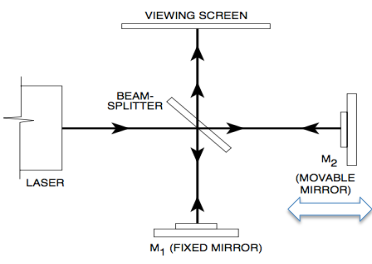
\includegraphics[width=0.5\textwidth]{michelson-interferometer/michelson-schematic.png}
	\caption{Schematic of a Michelson interferometer.}\label{mi:fig:schematic}
\end{figure}

In this way the original beam of light splits, and portions of the resulting beams are brought back together. The
beams are from the same source and their phases are hence highly correlated. When mirror $M_2$ is moved (closer to or
further from the laser source) the \textit{difference} in the path length of the light beams $(B$M$_1 - B$M$_2)$ changes, resulting in
changed in interference fringes. For a clear visualization of the effect, a lens placed between the laser source and the
beam-splitter spreads out the beam. An interference pattern of dark and bright rings, or \textit{fringes}, is seen on the
viewing screen. The rings are generated by interference of different portions of the laser beam, expanded to easy
visibility by the lens.

\section{Setup and Alignment of the interferometer}

Before you do an experiment with the interferometer, you'll need to ensure that it is aligned and an interference pattern (a set of concentric alternating light and dark rings) is clearly seen on the viewing screen when the laser is turned on. If that's true, then you can skip ahead to the next section.

Our laboratory setup is shown in Figure~\ref{mi:fig:setup-photo}.

\begin{framed}
	\textbf{Warning: Laser Hazard!} Lasers can cause temporary and permanent damage to eyes when exposed directly or through reflective surfaces.
	
	The following rules reduce the risk of eye exposure to laser light:
	\begin{enumerate}
		\item Do not direct the laser beam into anyone's eye.
		\item Be aware of the laser reflecting off of mirror-like surfaces and where that beam goes.
		\item Turn off the laser when not in use.
		\item Keep the laser pointing horizontally and near the plane of the table, while keep your eyes above that plane.
		\item To determine whether the laser is on, put your hand or a light-colored object in front of the beam, rather than looking into the laser aperture.
	\end{enumerate}
\end{framed}

\begin{figure}
	\centering
	\includegraphics[width=\textwidth]{michelson-interferometer/setup-photo.png}
	\caption{Our particular classroom setup, fully assembled and aligned, showing an interference pattern on the viewing screen.}\label{mi:fig:setup-photo}
\end{figure}

\begin{enumerate}
	\item The interferometer itself (this is part that has the optics) should be bolted to an optical rail at one end, with the
beamsplitter mirror facing the long end of the rail. Do so, if this isn't already in place.

	\item An aluminum block, with upward
facing magnets, should also be bolted into the rail near the other end.

	\item A steel plate, with an upturned edge, should
also be bolted to the rail, with the flat edge tight against edge of the interferometer.

	\item A 3⁄4” thick steel block, with two V-shaped grooves (one large and one small) should be placed on top of the aluminum block with magnets, with the V-shaped grooves facing upward; the magnets will keep the steel block in place.
	
	\item To begin, orient the block so the V-shaped grooves are aligned with the long axis of the rail, and the larger groove is toward the side of the rail opposite from the position of M$_1$ in the interferometer. The grooves are mount points for lasers, of two different barrel widths.
	
	\item Place a laser in one of the V-shaped grooves, pointed toward the interferometer, and turn it on. If necessary, you may secure the laser to the block using an elastic band or similar, taking advantage of the small grooves on the underside of the block that allow easy passage of a securing band.
	
	\item Place a viewing screen so that it is opposite M$_1$, or use a convenient light-colored wall.
	
	\item Loosen the thumbscrew that holds the beam-splitter and rotate the beam-splitter so it is out of the beam path of the
	laser as shown in Figure~\ref{mi:fig:adjusting-m1}.
	
	\begin{figure}
		\centering
		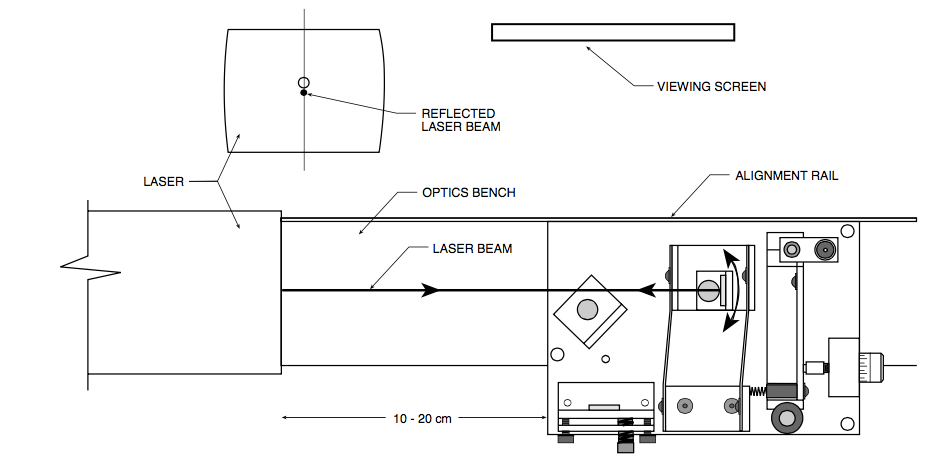
\includegraphics[width=\textwidth]{michelson-interferometer/adjusting-m1.png}
		\caption{Adjusting the M$_1$ mirror.}\label{mi:fig:adjusting-m1}
	\end{figure}
	
	\item Align the steel block holding the laser so that the beam hits M$_2$ as well-centered as
	possible; you can slide the steel block, rotate it (the magnets hold it in place but allow freedom of movement), and place paper in the groove under the laser to adjust the height or angle.
	Your goal should be to have the laser beam parallel to the long axis of the optical rail, and centered on M$_2$.
	
	\item The reflected beam should return back to the laser head. (The reflected beam need not be --- and likely won’t be --- at the
	same height as the incident beam, but it should return along the same path when viewed from exactly above. Hold
	your hand or piece of paper near the laser head --- without blocking the outgoing beam --- to see where the return beam
	is going.) If the return beam is not going where you want, you may loosen the thumbscrew that holds M$_2$ and adjust
	the rotation of M$_2$ so the laser beam is reflected directly back toward the laser head. Once satisfied with the alignment,
	hold M$_2$ in position and tighten the thumbscrew.
	
	\item Adjust the alignment screws on the mount for the mirror M$_2$, so that the mount plate does not appear tilted (see Figure~\ref{mi:fig:aligning-spots} for the location of these screws). When viewed from above there is gap between the plate holding the mirror and a
	second plate behind it. Adjust the screws so the plates appear parallel.
	
	\begin{figure}
		\centering
		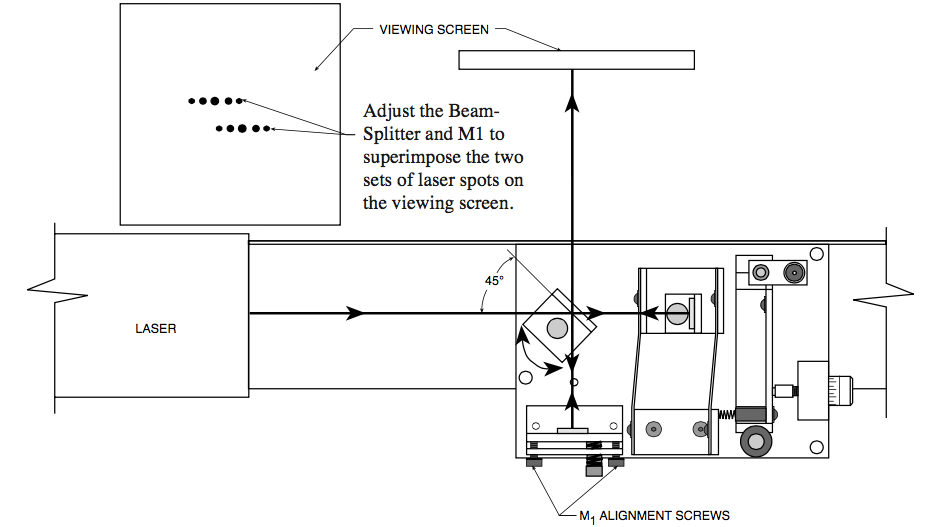
\includegraphics[width=\textwidth]{michelson-interferometer/aligning-laser-spots.png}
		\caption{Aligning the laser spots.}\label{mi:fig:aligning-spots}
	\end{figure}

	\item Rotate the beam-splitter so its surface is at an angle approximately 45 with the incident beam from the laser (see Figure~\ref{mi:fig:aligning-spots}). You will see two sets of laser spots on the viewing screen, corresponding to the two paths that the beam takes in reaching the screen. (Each path results in more than one laser spot because of multiple reflections within the beam-
	splitter.) Adjust the beam-splitter so the two sets of laser spots are as close as possible, then tighten the thumbscrew
	to secure the beam-splitter.
	
	\item Now, using the alignment screws, adjust the angle of M$_1$ until the two sets of laser spots are superimposed on the
	viewing screen (the two brightest spots must be superimposed).
	
	\item Place the 18 mm focal length lens on the optical bench on the steel plate between the laser mount and the
	interferometer (see Figure~\ref{mi:fig:positioning-lens} for setup and resulting desired pattern). The lens is in a holder that is magnetically coupled to a base; align one long edge of the base along the
	upturned edge of the steel plate. The lens should be about 10cm from the beamsplitter. Adjust the position of the lens
	on the holder so the light from the laser, now spread out by the lens, strikes the center of the beam-splitter. Move the
	lens vertically by sliding the lens holder vertically against the base (the magnets again allow freedom of movement
	here. The simplest way to move lens horizontally is to just slide the base lone the edge of the steel plate below. You
	should see an illuminated oval (or at least a partially illuminated oval) of laser light on the viewing screen. Adjust the
	lens position until the oval is as uniformly illuminated as you can achieve. Now, if you have performed the alignment
	correctly, you will see not just an illuminated oval, but a interference pattern of concentric rings on the viewing screen.
	If the alignment is not just right, the center of the fringe pattern may not be visible on the screen. Adjust the alignment
	screws on M$_1$ very slowly as needed to center the pattern. \textit{NOTE: aligning the interferometer so that you get fringes
	can be fiddly...if necessary, try a few times, and seek help from your TA if you cannot make it work.}

	\begin{figure}
		\centering
		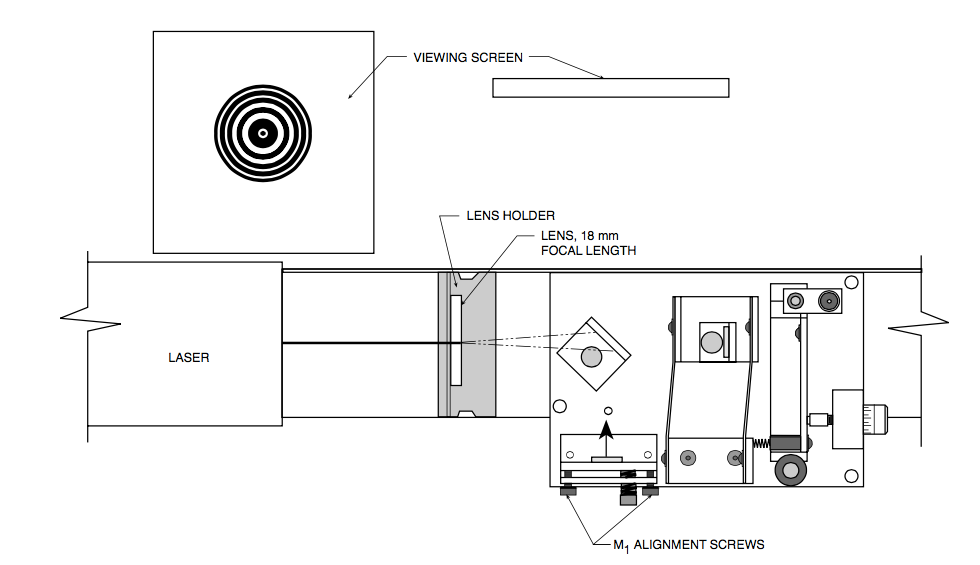
\includegraphics[width=\textwidth]{michelson-interferometer/positioning-lens.png}
		\caption{Positioning the lens, and fine alignment of M$_1$.}\label{mi:fig:positioning-lens}
	\end{figure}

\end{enumerate}

\section{Relating wavelength to distance changes}

By moving the mirror M$_2$, the path length of one of the beams can be varied. Since the beam traverses the path
between M$_2$ and the beam-splitter twice, moving M$_2$ 1/4 wavelength nearer to the beam-splitter will reduce the optical
path of that beam by 1/2 wavelength. The interference pattern will change; the radii of the maxima will be reduced so
they now occupy the position of the former minima. If M$_2$ is moved an additional 1/4 wavelength closer to the beam-splitter, the radii of the maxima will again be reduced so maxima and minima trade positions. However, this new
arrangement will be indistinguishable from the original pattern. So when moving the position of M$_2$, you will observe the
fringes ``moving'' reproducing the original pattern.

The movement distance $d$ of the mirror M$_2$ and the corresponding number of times $m$ the fringe pattern is restored to its original state are related by
\begin{equation}\label{mi:eq:interference}
 m \lambda = 2 d \, ,
\end{equation}
where $\lambda$ is the wavelength of the incident light. Thus, very small displacements d can be measured by counting the number m. Conversely, the wavelength of the light
can be accurately determined if d is known. In your interferometer, a knob with a micrometer scale can be used to move
M$_2$. M$_2$ is help on a lever spring arm that is anchored to the baseplate of the interferometer at another location. The
micrometer knob pushes on another arm that applies tension to a strap that is coupled to the lever arm holding M$_2$.

\section{Experiment 1: determining the wavelength of the laser}

\textbf{Goal:} Determine the wavelength of a laser.

\textbf{Rubric rows to be assessed:} D1, D4, F1, F2, G2, G4, G5.

\textbf{Available equipment:} Michelson interferometer mounted on optical rail, laser

Since this is such a sensitive measurement, we provide a measurement procedure for you. In order to determine the wavelength, you'll measure the number of fringes moved and the distance the mirror moved  and use Equation~\ref{mi:eq:interference} to calculate the wavelength of the laser.

\subsection{Procedure}

\begin{enumerate}
	\item\label{mi:step:micro} Adjust the micrometer knob so the lever arm is approximately parallel with the short edge of the interferometer
	baseplate. In this position the relationship between knob rotation and mirror movement is most nearly linear.
	
	\item Turn the micrometer knob one full turn counterclockwise. Continue turning counterclockwise until the zero on the
	knob is aligned with the index mark. \textit{(NOTE: Whenever you reverse the direction in which you turn the micrometer
	knob, there is a small amount of give before the mirror begins to move. This is called mechanical backlash, and is
	present in any mechanical system involving reversals in direction of movement. By beginning with a full
	counterclockwise turn, and then turning only counterclockwise when counting fringes, you can eliminate backlash
	in your measurement.)}

	\item Place a sheet of paper on the viewing screen, secure it with tape, and make a reference mark on the paper between
	two of the fringes. This will help you in keeping count of the fringes.
	
	\item Now turn counterclockwise the knob until you have counted about 40 movements of the fringes.
	
	\item\label{mi:step:record} Record the measurement on the knob as distance $d$ and record the number of fringe movements $m$.
	
	\item Repeat Steps~\ref{mi:step:micro}--\ref{mi:step:record} 2 more times, for a total of 3 measurements.
\end{enumerate}

Use your findings to determine the wavelength of the laser, including an estimate of the uncertainty in your reported value. Include the following in your report:
\begin{enumerate}
	\item A statement of the problem you are solving (D1).
	
	\item A clear, concise description of the experimental setup and procedure (F1).
	
	\item A table of the data that you took (G4).
	
	\item A description of your analysis that led you to find the wavelength (G5).
	
	\item A description, with calculations shown, of your determination of the uncertainty in the wavelength (G2).
	
	\item A final judgment of what your team thinks the wavelength of the laser is, based on your experimental results, including uncertainty (D4).
	
	\item A discussion of the findings of the experiment and why it's helpful (for you and/or for science) (F2).
\end{enumerate}

\section{Experiment 2: Measuring distance changes}

In your individual homework, you will determine distance changes in one of the arms of the interferometer, not caused by gravitational waves, like in LIGO, but by thermal expansion and the slight bending of the baseplate of the apparatus. During lab, take the following data, both without turning the knob to move the mirror:

\begin{enumerate}
	\item The clear strap that pulls the mirror back and forth will expand and contract with heating and cooling (like most solids). Measure the number of fringe movements that happen when you hold your finger very close to the strap, within a few millimeters, for 20--30 seconds.
	
	\item The baseplate is very sturdy, yet still bends when uneven pressure is applied, even if imperceptible to our senses. Measure the number of fringe movements that happen when you press lightly on the baseplate between one of the mirrors and the beam-splitter.
\end{enumerate}

\section{Individual homework}

\begin{enumerate}
	\item Use the data taken during Experiment 2 to determine the path length changes in each case (include calculation of uncertainty).
	
	\item Report on if this is surprising to you or not, either that the distance change is as large or small as it is, or the fact that you can measure such a small distance change.
	
	\item For what useful or fun purpose could this kind of sensitive measurement technique be used?
\end{enumerate}

\chapter{Black hole at the Galactic center? (stellar orbits)}

%TODO replace homework with actually doable and physical arguments
%TODO restructure lab to make sense, be clear, organized
%TODO make equal-area section length^2, not arcsec^2

\section{``Observing'' Black Holes}

Black Holes are robustly predicted by Einstein's theory of General Relativity, the current state-of-
the-art in mathematical explanations of gravitational phenomenon. It has also been demonstrated
theoretically that such extreme objects naturally arise in the late-stages of stellar evolution for the
most massive stars. However, they are difficult to observe for a simple reason: by their very nature (as
suggested by their name), they do not emit light. Nonetheless, their presence can be inferred indirectly
through their gravitational effect on other objects. Astronomers and physicists have discovered so many
independent and corroborating lines of evidence of this type detected that the existence of black holes
is now considered a well-established scientific fact.

The detection of gravitational waves by the Laser Interferometer Gravitational-Wave Observatory
(LIGO) in 2017 is arguably the most stunning and conclusive evidence of this to date. In a
beautiful demonstration of the validity of General Relativity, the perturbations in space and time
(Gravitational Waves) characteristically generated by the coalescence of a binary black hole pair were
detected on Earth after having traveled at the speed of light from their source roughly one billion light
years away. The clarity of this signal and its agreement with predictions have all but conclusively
determined the existence of black holes.

However, less direct (but nonetheless extremely convincing) evidence for the existence of black holes
had been well known in observational astronomy for some time. In this lab, you will explore one of the
most striking examples of these observational signatures: the orbits of stars around Sag A*, the radio source that is collocated with the `dark attractor' at the center of our galaxy that is almost certainly a Super-Massive Black Hole (SMBH). Astronomers now know that almost all galaxies have such behemoths at their centers, and that they likely play a fundamental role in galaxy evolution. The discovery of one at the center of the Milky Way (roughly 8 kpc distant) was an important step in the development of this SMBH paradigm. In this lab, you will partially reproduce a simplified version of the analysis that led astronomers to this exciting conclusion.

\textbf{Rubric Rows to be assessed:} C4 and C5 (for Kepler's 2nd Law); D8, D9, and G1 (for Kepler's 3rd Law mass estimation); F1 and F2 (for all parts)

\section{Newtonian Dynamics and Orbital Dynamics Basics}

The trajectories of objects moving under the influence of gravity are generally called \textit{orbits}. Newton's
Law of Gravity, while not an adequate description for extreme gravitational fields, is nonetheless a good
approximation generally and in the specific cases of orbits we'll be examining. It is given by
\begin{equation}\label{gc:eq:newton}
 F_\textrm{grav} = G \frac{m_1 \: m_2}{r^2} \, ,
\end{equation}
where $F_\textrm{grav}$ is the force of gravity between any two objects of mass $m_1$ and $m_2$ a distance $r$ from each other. $G$ is Newton's Gravitational Constant, whose value in CGS (Centimeters Grams Seconds) units
is $6.67 \times 10^{-8}\:\textrm{cm}^3 \: \textrm{g}^{-1} \: \textrm{s}^{-2}$. The gravitational force is attractive: it pulls objects together. This, coupled
with Newton's Second Law of Motion relating the force acted upon an object $F$ and its acceleration $a$,
\begin{equation}
 F = ma \,,
\end{equation}
tells us that \textit{the acceleration of an object due to gravity will be greater in stronger gravitational fields}.
These two fundamental physical laws can be used to derive the properties of Newtonian gravitational
orbital motion. We won't do so here, but instead just cover some of the key implications, concisely
stated by Kepler's Laws of Orbital Motion. These Laws, which are concise mathematical descriptions
of how the planets move in the Solar System, preceded Newton's work by nearly a century, and were
based solely on observational data. Newton's work on gravity and motion explained, at a deeper level,
why Kepler's Laws are as they are.

\subsection{Kepler's Laws}

\subsubsection{Kepler's First Law}

Kepler’s First Law states that \textbf{A planet orbits the Sun in an ellipse, with the Sun at one focus
of the ellipse.} This is true generally for any mass orbiting a much more massive object. An \textit{ellipse} is a
generalization of a circle, allowing for the circle to be stretched along a certain direction. See Figure~\ref{gc:fig:ellipse} for details.

\begin{figure}
	\centering
	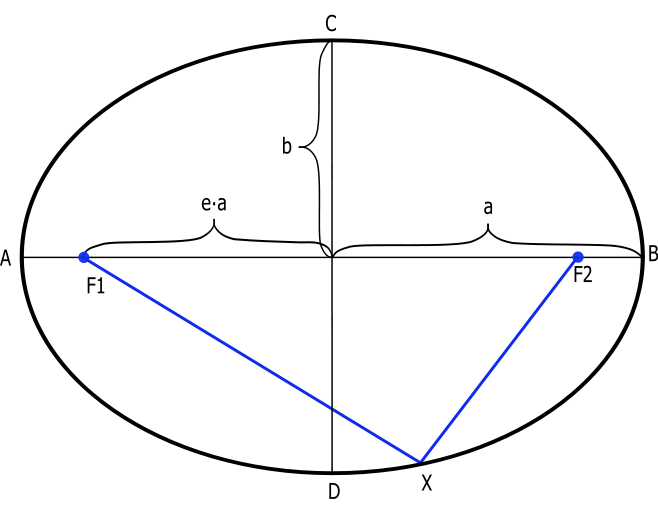
\includegraphics[width=0.6\textwidth]{galactic-center/ellipse.png}
	\caption{The geometry of an ellipse: $a$ is the semi-major axis of the ellipse, F1 and F2 are each a
		focus of the ellipse, $b$ is the semi-minor axis, and $e$ is the eccentricity. The eccentricity describes
		the extent to which the ellipse is oblong: an ellipse with $e = 0$ is just a circle. The foci are defined such
		that the distance from F1 to X, added to the distance from F2 to X, is the same no matter where X
		is located on the ellipse. For a circle, the foci coincide at the center. The Newtonian generalization of
		Kepler's First Law tells us that a small mass will orbit a much larger mass on an ellipse, and the larger
		mass will be located at one of the foci.}\label{gc:fig:ellipse}
\end{figure}

\subsubsection{Kepler's Second Law}

The second law states that \textbf{a line connecting a planet to the Sun sweeps out equal areas in
equal time intervals}. This concept is demonstrated in Figure~\ref{gc:fig:keplers-2nd-ellipse}. As a consequence of this, when a
planet is closer to the sun, it orbits with a faster velocity. Furthermore, planets that have more circular
orbits will have more uniform velocities over the course of their orbit than those with very eccentric
orbits.

\begin{figure}
	\centering
	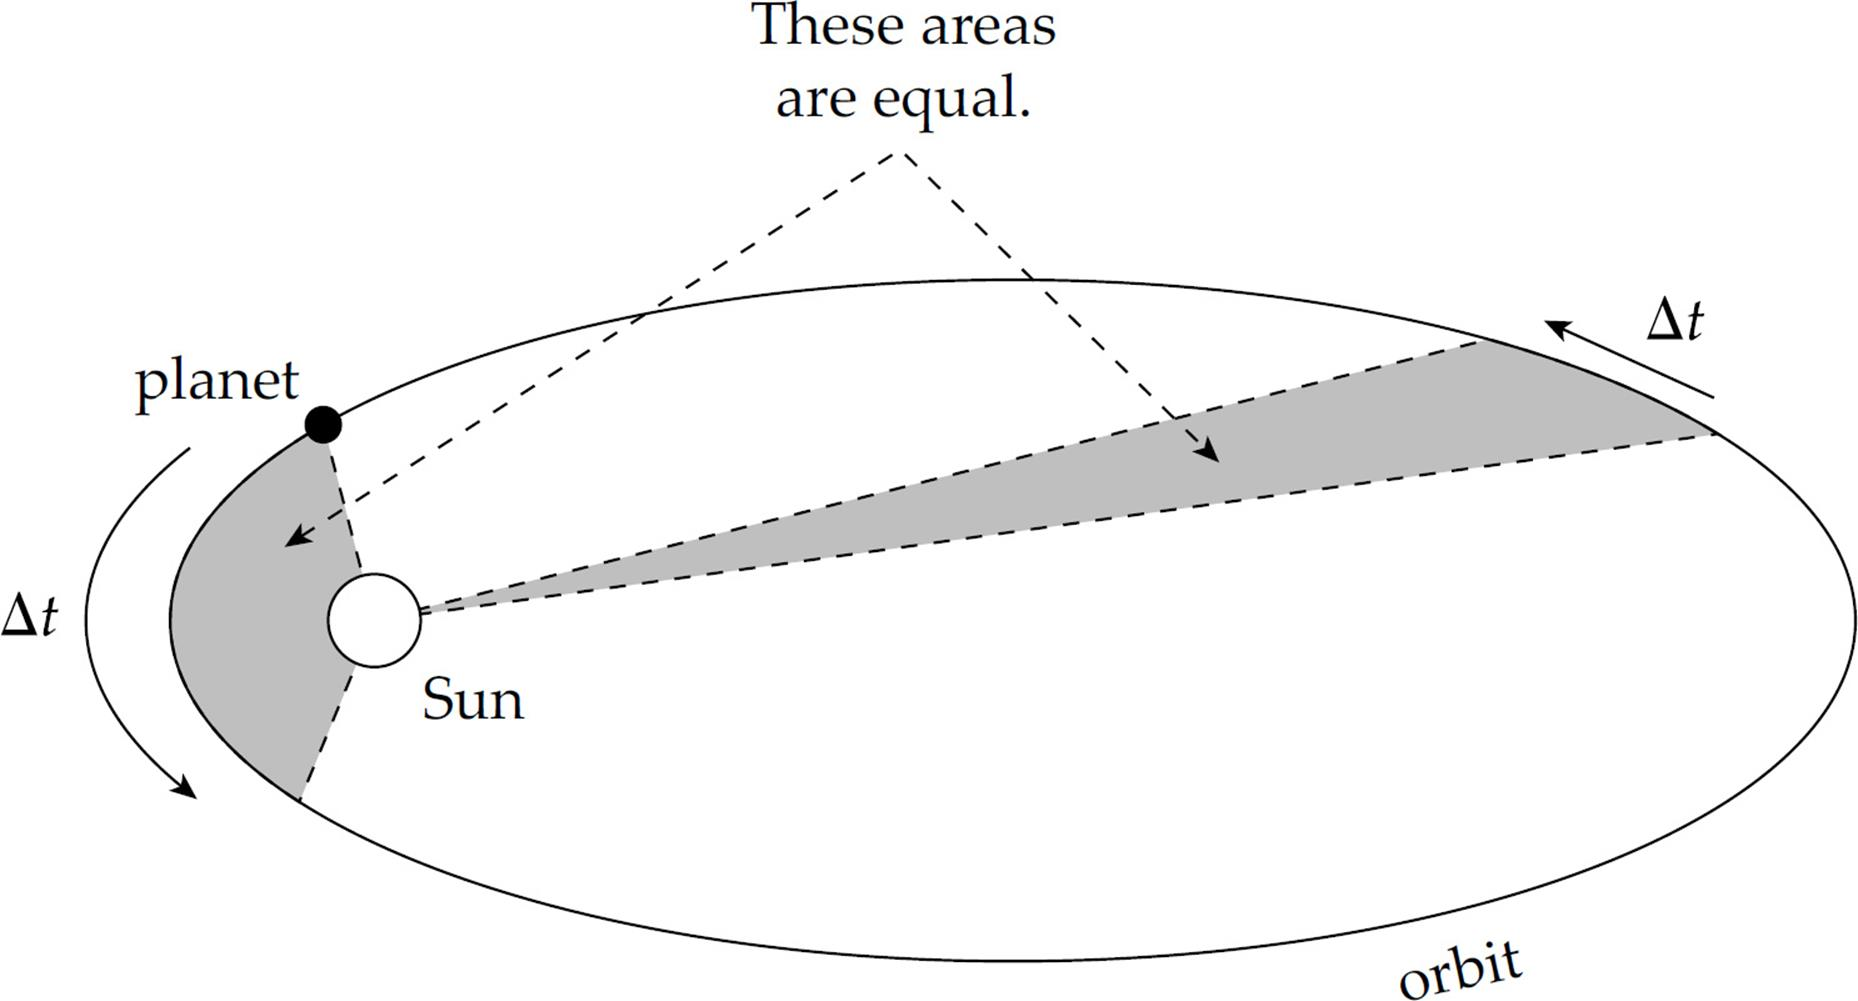
\includegraphics[width=0.7\textwidth]{galactic-center/keplers-2nd-ellipse.png}
	\caption{Illustration of Kepler’s Second Law. The shaded regions are of equal area, so by Kepler’s Second Law, the
		planet passes through each region of the orbit in the same amount of time. Since the region of the orbit
		where the planet is closest to the Sun is a much further distance, and speed is change in position over
		change in time, the planet will move with a much faster average speed than at the other portion of the
		orbit, far away from the sun.}\label{gc:fig:keplers-2nd-ellipse}
\end{figure}

\subsubsection{Kepler's Third Law}

Kepler’s Third law addresses the path of an object $m$ as it orbits a much more massive object of mass $M$. Specifically, it relates the orbital period $P$ (the time it takes for one complete orbit to occur) to the semi-major axis $a$ of the ellipse according to
\begin{equation}\label{gc:eq:kepler-3}
 P^2 = \frac{4 \pi^2}{G M} a^3 \,,
\end{equation}
where other objects are also considered to be not affecting the orbit of $m$. \textbf{This is the
	equation you will be using in the central calculation of the lab.}

An important qualification to be made about Kepler’s Laws is that they apply only to two-body
systems. Kepler’s Third law breaks down when you have more than 2 orbiting objects in a system.
However, they are nonetheless a very good approximation for the orbits of small masses around a much
larger mass, in which case the gravitational force of the massive object dominates over the intra-small-
object interactions, and thus each smaller body approximately behaves independently from the other
small objects. And so the motion of each small object, to a good approximation, can be modeled by
Kepler’s Laws.

\subsection{Escape speed}

Another important concept in orbital dynamics --- which comes from the general Newtonian understanding of orbits --- is that of the escape speed. This is the minimum speed that an object must reach
to break out of its orbit at a certain radius from the central massive object. The escape speed $v_\textrm{escape}$ at a
distance $r$ from the center of a mass $M$ is given by
\begin{equation}\label{gc:eq:escape-speed}
 v_\textrm{escape} = \sqrt{\frac{2 G M}{r}} \,.
\end{equation}
An orbiting object that achieves a speed greater than this is unbound to the object it is orbiting, and will escape its gravitational pull, flying out of the system entirely.

\section{General Relativity}

Despite the great success of Newtonian dynamics in explaining a wide variety of the celestial motions
that we observe, this picture of gravity is incomplete and inaccurate in the most extreme regimes,
where General Relativity is required. A fully self-consistent description of relativity is well beyond the
scope of these notes (or this course), but the fundamental conceptual premise is easily stated: gravity
is not a magical “attraction at a distance” between objects with mass, but rather the result of curved
space-time, which is an effect of all mass. A helpful analogy is that of a sheet of fabric being depressed
by a massive object (see Figure~\ref{gc:fig:gen-rel-sheet}). Other objects placed on this depressed fabric will begin orbiting
around the massive object.

\begin{figure}
	\centering
	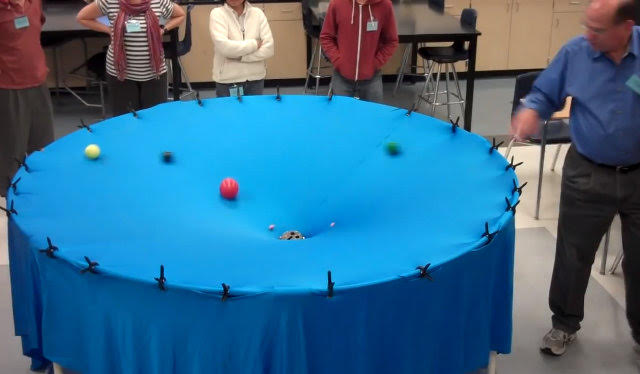
\includegraphics[width=\textwidth]{galactic-center/gen-rel-sheet.png}
	\caption{General Relativity Analogy.}\label{gc:fig:gen-rel-sheet}
\end{figure}

For the purpose of this lab, the most important consequence of this paradigm shift is the fact that
gravity thus affects everything, including even massless objects like light, in exactly the same way that
it does massive objects, since they also travel through space-time. Thus, there might exist objects with 
such extremely strong gravitational fields (and thus extremely contorted spacetimes) that even light
cannot escape. Since Special Relativity (Einstein’s original theory of relativity, which he later built
off of to develop General Relativity) tells us that light sets the cosmic speed limit, nothing else can
escape either. These are termed Black Holes. We should note that, while we are assessing observational
evidence for a black-hole in this lab, we will nonetheless use the Newtonian gravitational framework to
understand our observations, sine the gravitational fields experienced by the stars we are observing are
--- to an excellent approximation --- well-described by Newtonian gravity.

\section{Schwarzschild Radii}

One can extend Newtonian dynamical arguments to estimate the relevant scales for relativistic objects.
For example, in the context of Newtonian Gravitation, one can think of a Black Hole as an object that
has an escape velocity greater than the speed of light. Thus one can substitute the speed of light into
the equation for the escape speed (Equation~\ref{gc:eq:escape-speed}) to estimate the radius of a Black Hole,
\begin{equation}
 R_\textrm{Schwarzschild} = \frac{2 G M}{c^2} \,
\end{equation}
where $c = 2.998 \times 10^{10}\:\mathrm{cm}/\mathrm{s}$ is the speed of light. $R_\textrm{Schwarzschild}$ is called the Schwarzschild Radius, and is actually the correct value predicted by General
Relativity for a certain class of black holes, so it’s a very good estimate. Any object dense enough to be
contained inside of its Schwarzschild radius must be a black hole.

\section{Lab Tasks}

For each of the following objects, a) calculate the Schwarzschild radius for that object’s mass, b) list
an everyday object of comparable size and c) find the ratio of the Schwarzschild to physical radius of
the object: (hint: do this in excel so you don’t have to repeat the calculation \textit{ad nauseum})
\begin{enumerate}
	\item One of your group members.
	\item the Earth.
	\item the Sun.
	\item the Solar System.
	\item The Milky Way Galaxy.
\end{enumerate}

\section{Orbit Simulator and 3D model}

First we will explore some interactive animations of orbital motion, then a three-dimensional rendering
of the real scientific data that we will analyze in the second part of this lab.

\section{Lab Tasks}
\begin{enumerate}
	\item Go to
	
	\url{https://www.windows2universe.org/physical_science/physics/mechanics/orbit/orbit_shape_interactive.html}. This website allows one to adjust the shape of an orbit for a hypothetical planet in the solar system.

	\begin{enumerate}
		\item Set the semi-major axis at 1AU (the radius of Earth’s nearly-circular orbit), and the eccentricity to it’s maximum value (0.9). By observing the motion of the planet with respect to
		Earth, verify (qualitatively, no need for numerical calculations here) each of Kepler’s Three
		Laws.
		
		\item Based on the orbital dynamics your observe, what simplifying approximations can you tell
		are being made in the calculation that goes into this animation? Particularly notice when
		your test planet comes close to another planet in its orbit. Do their orbits remain the same?
		Should they?
	\end{enumerate}

	\item Now go to \url{www.astro.ucla.edu/~ghezgroup/gc/animations.html}, the website for the UCLA
	Galactic Center Group, where you will find a number of informative graphics that relate to the
	content of this lab. On the bottom-right under the section “3D Movie of Stellar Orbits in the Central Parsec” is a volume-rendered video of stars orbiting Sag A* --- the radio and X-
	ray source at the center of the galaxy, the mass of which you will be measuring in the next
	section.
	
	\item Expand the video to full-screen and pay attention to one or two of the stellar orbits,
	which are show in full by the video. Pause the video at several points during the video. How
	do the 2D shapes of the orbits on the image change as the camera angle moves? How does the
	inclination of the orbital plane in our field-of-view modify the observed orbital shape? How might
	this confuse the determination of orbital parameters? How can we disentangle this? (hint: think
	about Kepler’s Laws and the location of the foci). What kind of errors in our measurement will
	result from an assumption that we are looking at an orbit directly from above? Will this cause the inferred mass to be over- or under-estimated? (See Scientific Ability Rubric Row D9 in Table~\ref{rubric:d}).
	
	\item As well, consider the spatial orientation of the orbits here with reference to those of the solar
	system, considered in the previous task. Is there any coherent organization of stellar orbits
	around the black hole in this video? How does this compare to the orientation of planets in
	the solar system? What might be a physical reason for this difference (hint: think about their
	respective formation mechanisms).
\end{enumerate}

\section{Sag A* Mass Estimation}

Now you will roughly measure the mass of Sag A* by extracting the positions of several stars orbiting
the galactic center from a published YouTube video that illustrates the stellar dynamics observed by
the UCLA Galactic Center research group. Their data comes from the largest research telescopes on
the planet, observing the Galactic Center using sophisticated imaging cameras that give images even
sharper than those produced by the Hubble Space Telescope. We will ”observe” the video of their
measurements, to illustrate the process of data → measurement → analysis → conclusion (a mass!).

\subsection{Lab Tasks}

\begin{enumerate}
	\item Go to \url{https://www.youtube.com/watch?v=7vcSKbXnLJA}. This movie shows observations of Sag
	A* and the surrounding stellar cluster taken over more than a decade. Watch the video, and record
	your impressions in light of your previous activities on orbital dynamics and the introductory
	information. What is going on here? How might this be used as evidence for the existence
	of a SMBH at the galactic center? What other corroborating data would you want/need to
	substantiate that claim?
	
	\item After watching several times and recording your initial impressions, you will now take some crude “measurements” of the data in the video. You will then use these to both verify Kepler’s Second Law and make an order-of-magnitude estimate of Sag A*’s mass using Kepler’s Third Law.
	
	Data acquisition:
	\begin{enumerate}
		\item Restart the video and take a screen-grab of the first frame using the PrintScreen function (you will
		be doing this several times so make a folder in which to save your screenshots).
		
		\item Let the animation advance by one second (so that the stars have begun moving in their
		orbits), pause, and capture another screen image. Do this for each second of the animation,
		giving you 9 separate images of the stars in different positions on their orbits.
		
		\item For Kepler's Second Law, you will need to measure several areas traced out by an orbit in the same time duration. Open the first frame in the ImageJ software. Note the white arrow on the left of the
		screen indicating the angular scale of the image.
		%Notice that Kepler's law describes areas, while we are limited, at present, to angular areas, since we are not including how far away the stars are to us. This approximation should be just fine for testing the law, as long as the angle is small.
		
		\item On the menu tab click the straight line icon
		located at the 5th position to the left. Click one end of the arrow and drag the line from one
		end of the angular scale to the other. Now go to the Analyze dropdown menu and select Set
		Scale. Set the known distance to be the distance of the scale, 0.1 arcseconds. (Look up how
		to convert from arcseconds to degrees, and then to radians).
		
		\item Once the scale is set, select the straight line icon again and drag the line from the star symbol
		(representing Sag A*) to the orbiting star you want to measure. The measure hotkey is ”m.”
		This will now give you the angular distance from Sag A* to the orbiting star in arcseconds.
		It will also give you an angle value that will allow you to measure the angular rotation of
		the star in its orbit. Record these values for both S0-2 and S0-37 in the first 2 columns of a data table set up like Table~\ref{gc:tab:orbits}, one table for each of these stars, one row for every frame you captured.
		
\begin{table}
	\centering
	\begin{tabular}{c|c|c|c|c|c}
		frame & $d$ (arcseconds) & $s$ (cm) & $\theta$ (radians) & $\Delta \theta$ (radians) & $A$ (cm$^2$)
		\\ \midrule
		1 & & & & \cellcolor{black!25} & \cellcolor{black!25}
		\\ \midrule
		2 & & & & & 
		\\ \midrule
		3 & & & &  &
		\\ \midrule
		4 & & & &  &
		\\ \midrule
		5 & & & & &
		\\ \midrule
		6 & & & & &
		\\ \midrule
		7 & & & & &
		\\ \midrule
		8 & & & & &
		\\ \midrule
		9 & & & & &
		\\ \bottomrule
	\end{tabular}
	\caption{Data table for one stellar orbit. Note that you will not have any calculations for the gray cells for frame 1, since there is no previous frame to compare to.}\label{gc:tab:orbits}
\end{table}		

	\end{enumerate}

	\item Kepler's Laws:
	\begin{enumerate}
		\item Kepler's Second Law: This data can now be used to test Kepler’s Second Law. The area
		covered by a line connecting the planet and Sag A* between measurements $i$ and $i - 1$ can
		be given by
		\begin{equation}
		 A_i = \pi \left( \frac{s_{i} + s_{i-1}}{2} \right)^2 \left( \frac{\theta_{i}-\theta_{i-1}}{2\pi} \right) \,,
		\end{equation}
		which approximates the swept area as the sector of a circle. To compute the distances $s_i$ from the angular distances $d_i$, convert $d$ to radians and multiply by the distance to Sag A*, $2.47 \pm 0.05 \times 10^{22}\:$cm.  Add this calculation for each
		segment and both stars to the data table. Does Kepler’s Second Law hold? Discuss any
		discrepancies and how you might account for them (Rubric Rows C4, C7, C8).
		
		\item Kepler’s Third Law: Now you will use Kepler’s Third Law, given in the introduction, to
		calculate the central mass around which these objects are orbiting. Go back to the final
		frame of the video and use the traced orbits to estimate the semi-major axis for both S0-2
		and S0-37. This estimated length is an angular length in arcseconds and should be converted to a physical length in centimeters. First convert the arcseconds to radians, then multiply it by the distance from Earth to Sag A*, and use the timestamps on
		the video to estimate the orbital periods in seconds. Note that, while this is straightforward for S0-2
		since it completes a full orbit in the span of the video, this is less obvious for S0-37. The
		key here is that S0-37 has a circular orbit. Use Kepler’s Laws and the previous discussion of
		oribital inclination observational effects to determine how S0-37’s period can be estimated
		from the given data. What approximations and assumptions need to be made to justify the
		use of this equation for the system we’re observing (Rubric Rows D8, D9)?
		
		\item Once you have done this calculation, compare your obtained value of M to the best-estimate
		mass of the central SMBH of $M_\mathrm{bh} = 4.0 \times 10^6\:\textrm{M}_\textrm{\astrosun}$ (Boehle \textit{et al.} 2016). How far off was your
		estimate? Was it within your estimated error (See Section~\ref{unc:sec:comparing})? List all possible sources of error and bias,
		both procedural and physical, in this calculation. Particularly, think about the applicability
		of Kepler’s Third Law to the physical system we are measuring (Rubric Rows G1, G2).
	\end{enumerate}

	\item Sag A* Size estimation
	\begin{enumerate}
		\item Now, that we have a mass estimate for Sag A*, the next step is to place upper limits on
		its physical size. Using the last frame in the video, try to use the paths of the orbits that
		come closest to the star symbol indicating Sag A* to place an upper limit on its radius. To
		determine that Sag A* is a black hole, we need to make an estimate of its physical extent,
		which will allow us to rule out all other plausible forms of matter (at least as far as we know).
		What is the physical value of this upper limit? Given the mass you calculated, how does
		this compare to its Schwarzschild radius?
		
		\item While this suggests that the central attractor is an extremely dense object, we can place
		even tighter constraints on its physical extent based on the timescales of its fluctuations
		in electromagnetic observation. Sag A* is lacking in any prominent optical emission, it is
		nonetheless observable in radio and X-ray frequencies. As well, we observe it’s brightness in
		these frequencies to flare (Figure~\ref{gc:fig:light-curve}) somewhat regularly on the order of once per day, with
		actual flare events lasting much less time. Since the speed of light is finite, when an object
		flares, light from the side of the object opposite the observer will become visible later than
		that from the side closest to the observer. Thus, the time it takes for the object to flare
		will be limited by light-travel time across the object. This allows us to use the light-travel
		distance over the timescale of the flare as an upper-limit on the physical extent of the object.
		Use Figure~\ref{gc:fig:light-curve} to do just this. Calculate the corresponding angular size of this distance as
		observed from earth (in arcseconds, for easy comparison with the video data). How does this
		measure compare with Schwarzschild radius of a black hole of the mass you measured?
		
		\begin{figure}
			\centering
			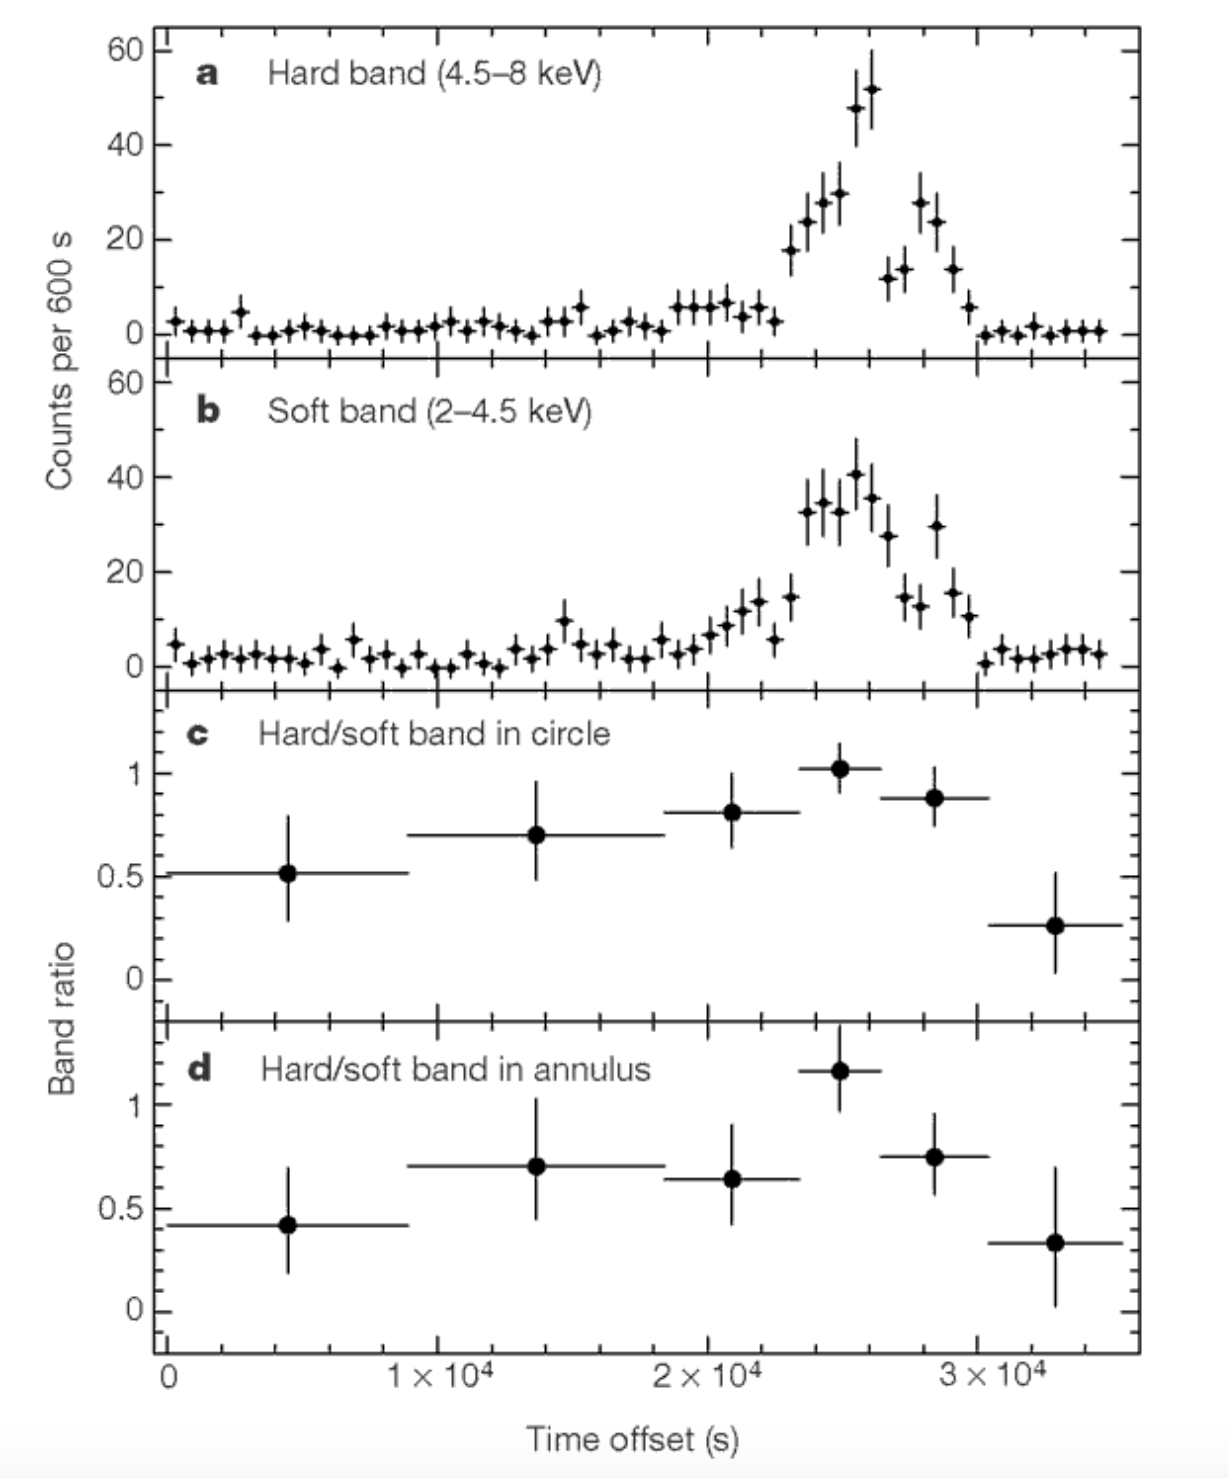
\includegraphics[width=0.7\textwidth]{galactic-center/sag-a-light-curve.png}
			\caption{Sag A* light curve, showing significant flaring on the timescale of a day.
				(from \url{https://heasarc.gsfc.nasa.gov/docs/objects/galaxies/sag-a star.html})}\label{gc:fig:light-curve}
		\end{figure}
	\end{enumerate}
\end{enumerate}

\section{Individual Homework}

There is no individual homework for this lab.

%Now that we have determined that Sag A* is an extremely dense, massive object --- but not quite certainly a black hole --- we are left to make plausibility arguments that allow us to
%eliminate all other possible forms of matter. For each category of astrophysical objects listed
%below, estimate the observational signatures of a hypothetical object with the mass you’ve
%measured for Sag A*. Decide whether or not the estimated observable properties can be used
%to rule out this alternative to a black hole.
%\begin{enumerate}
%	\item Main-Sequence Star/Cluster (Hint: the luminosity of massive stars scales as $M^4$, so
%	what luminosity would a Sag A*-star have? What would be the luminosity of a cluster
%	of sun-like stars with a total mass equal to that of Sag A*?)
%	
%	\item Brown Dwarf Star Cluster (Hint: A typical brown dwarf luminosity is $\sim 10^{-4} L_\textrm{\astrosun}$ and
%	the maximum brown dwarf mass is $0.08M_\textrm{\astrosun}$. Brown dwarfs more massive than this are
%	just stars, which you presumably ruled out above.)
%	
%	\item White Dwarf Star Cluster (Hint: a typical White Dwarf luminosity is $0.03L_\textrm{\astrosun}$, and the
%	maximum white dwarf mass is $1.4M_\textrm{\astrosun}$. There are fundamental physical arguments that
%	preclude the stable existence of a white dwarf above this mass.)
%	
%	\item Neutron Star Star Cluster (Hint: a typical Neutron Star luminosity is $10^{-6} L_\textrm{\astrosun}$ , and the
%	maximum neutron star mass is estimated to be $1.4M_\textrm{\astrosun}$. This maximum mass is also
%	derived from fundamental physics considerations). Would such a configuration, even if
%	hypothetically possible, be physically reasonable?
%\end{enumerate}
%\chapter{Black Hole at the Galactic Center?}

\section{Mystery at the Center of the Milky Way}
\begin{steps}
	\item Take a moment to watch the video found in the following link \url{www.astro.ucla.edu/~ghezgroup/gc/animations.html} under the heading \textbf{3D Movie of Stellar Orbits in the Central Parsec}.
\end{steps}
At first glance the video might not seem all too surprising as having learned about the solar system you likely expect orbiting planets to be a mundane fixture of the universe. However, what if you were to learn that the objects were not planets, but in fact stars and that what you see in the video spans a distance of 3 light years? For comparison, Pluto is only about .0006ly from the sun. In fact, the video you just saw is a visualization of a phenomenon in the center of our galaxy which puzzled astronomers for a long time. As you might have learned all objects exert a gravitational force which is proportional to the mass of the object. For this reason, smaller objects tend to be ``pulled in'' by larger objects, forming the orbital relationships we see in our daily lives: the moon orbiting the Earth, the Earth orbiting the Sun, and so on. Some of the most massive objects in the universe are stars which is why they tend to form the center of orbital systems. However, given that all the objects in the video were stars, this meant that there had to be a much, much more massive object in the center of our galaxy attracting them, one which seemed to be invisible, save for radio signals coming from the location of the object. There were many theories as to what the object, whose signal is dubbed Sagittarius A*, could  be. Some believed it to be a collection of massive objects such as stars or small black holes. The most compelling theory, however, was that thee source responsible for the signal was, in fact, a Supermassive Black Hole (SMBH).
Black holes are some of the most extreme objects in the universe which were first theorized to exist as a result of Einstein's theory of general relativity. In the most basic terms, a black hole is an extremely massive and dense object whose gravitational pull is so strong, that not even light can escape. This fact that light cannot escape from a black hole,  however, makes them incredibly difficult to observe directly. That said, due to the strength of their gravitational pull, black holes can often be detected indirectly based on their influence over nearby objects. In this lab you will examine the gravitational system you saw in the video and you will be able to determine whether the object in the center of the Milky Way is, in fact, a black hole. First, however, you will learn about the basic laws which govern orbital systems and how they can be applied to determine some of the physical properties of the objects in the system.

\section{Learning Goals}
\begin{itemize}
	\item Understand Kepler's laws of planetary motion and be able to use them to extract information about orbital systems.
	\item Be able to gather data using a variety of tools and understand the limitations of experimental data.
	\item Be able to make inferences about physical properties of objects which cannot be directly measured.
	\item Identify assumptions made during analysis and their effects on calculations.
\end{itemize}

\section{Installing ``ImageJ''}
For some parts of this lab you will be using a image analysis software called ``ImageJ'' to gather numerical data from images.
\begin{steps}
	\item Go to the following link to install the imageJ software \url{https://imagej.nih.gov/ij/download.html}
	\item Click on the link to the software version for your OS. This will download a .zip file.
	\item Once the file is downloaded, right click on the folder and choose ``extract all''. Once it is finished go into the folder you extracted the files to and click on the icon labeled ``Imagej''
\end{steps}

\section{Observation Experiment: Developing Orbital Dynamics Principles}
In general, an \textit{orbit} is what we call the path an object follows when under the gravitational influence of a larger mass. For the most part, the interactions between two gravitationally bound objects can be approximated using Newtonian mechanics, with the force of gravity between two objects given by 
\begin{equation}\label{gc:eq:newton}
	F_\textrm{grav} = G \frac{m_1 \: m_2}{r^2} \, ,
\end{equation}
where $m_1$ and $m_2$ are the masses of the two objects, $r$ is the distance between them, and $G$ is Newtons Gravitational Constant whose value is $6.67 \times 10^{-8}\:\textrm{cm}^3 \: \textrm{g}^{-1} \: \textrm{s}^{-2}$. This equation, coupled with Newton's Second Law of Motion $$F = ma$$ or force $F$ equals mass $m$ times acceleration $a$, tells us that the stronger the force of gravity, the greater the acceleration due to gravity. With these two fundamental principles, it is possible to derive many of the properties of orbital mechanics. Moreover, they allow us to understand the physics behind the mathematical description of orbits formulated by Johannes Kepler nearly a century earlier

\subsection{Kepler's Laws}
\subsubsection{Kepler's First Law}
Kepler's First Law simply states that \textbf{\textbf{A planet orbits the Sun in an ellipse, with the Sun at one focus of the ellipse.} This is true generally for any mass orbiting a much more massive object. An \textit{ellipse} (commonly referred to as an oval) is a generalization of a circle, allowing for the circle to be stretched along a certain direction. See Figure~\ref{gc:fig:ellipse} for details.}
\begin{figure}
	\centering
	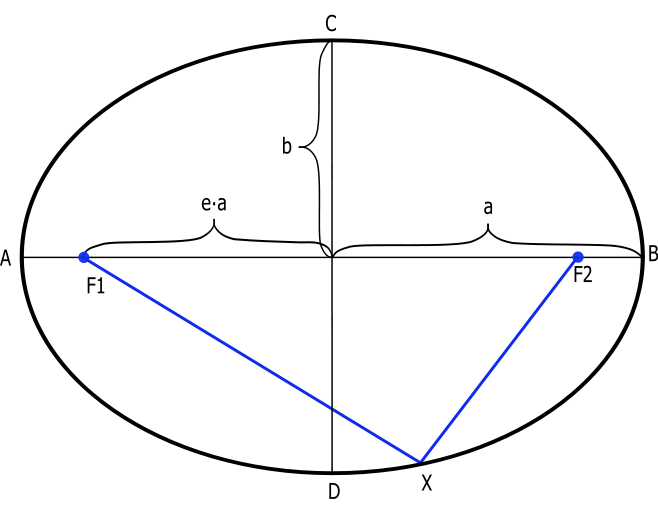
\includegraphics[width=0.6\textwidth]{galactic-center/ellipse.png}
	\caption{The geometry of an ellipse: $a$ is the semi-major axis of the ellipse, F1 and F2 are each a
		focus of the ellipse, $b$ is the semi-minor axis, and $e$ is the eccentricity. The eccentricity describes
		the extent to which the ellipse is oblong: an ellipse with $e = 0$ is just a circle. The foci are defined such
		that the distance from F1 to X, added to the distance from F2 to X, is the same no matter where X
		is located on the ellipse. For a circle, the foci coincide at the center. The Newtonian generalization of
		Kepler's First Law tells us that a small mass will orbit a much larger mass on an ellipse, and the larger
		mass will be located at one of the foci.}\label{gc:fig:ellipse}
\end{figure}
\subsubsection{Kepler's Second Law}
The second law states that \textbf{a line connecting a planet to the Sun sweeps out equal areas in
equal time intervals}. This concept is demonstrated in Figure~\ref{gc:fig:keplers-2nd-ellipse}. As a consequence of this, when a
planet is closer to the sun, it orbits with a faster velocity. Furthermore, planets that have more circular
orbits will have more uniform velocities over the course of their orbit than those with very eccentric
orbits.

\begin{figure}
	\centering
	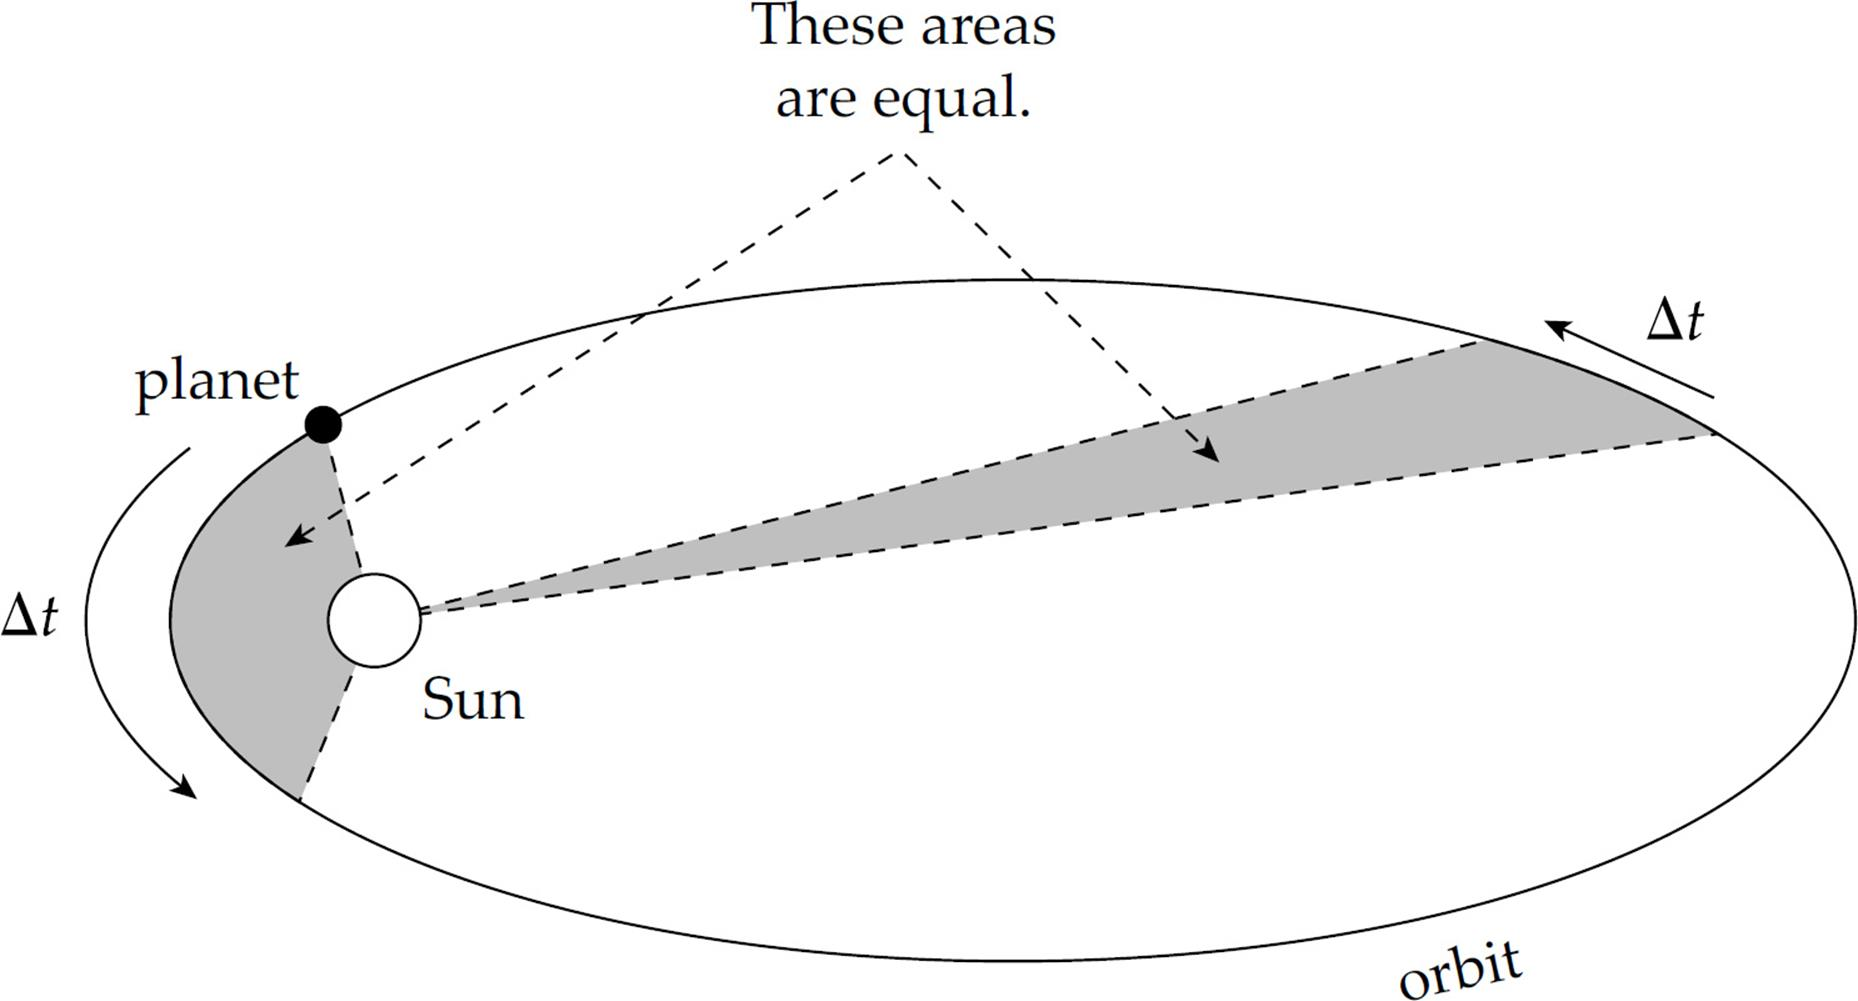
\includegraphics[width=0.7\textwidth]{galactic-center/keplers-2nd-ellipse.png}
	\caption{Illustration of Kepler’s Second Law. The shaded regions are of equal area, so by Kepler’s Second Law, the
		planet passes through each region of the orbit in the same amount of time. Since the region of the orbit
		where the planet is closest to the Sun is a much further distance, and speed is change in position over
		change in time, the planet will move with a much faster average speed than at the other portion of the
		orbit, far away from the sun.}\label{gc:fig:keplers-2nd-ellipse}
\end{figure}
\subsubsection{Kepler's Third Law}
Kepler’s Third law addresses the path of an object $m$ as it orbits a much more massive object of mass $M$. Specifically, it relates the orbital period $P$ (the time it takes for one complete orbit to occur) to the semi-major axis $a$ of the ellipse according to
\begin{equation}\label{gc:eq:kepler-3}
	P^2 = \frac{4 \pi^2}{G M} a^3 \,,
\end{equation}
where other objects are also considered to be not affecting the orbit of $m$. \textbf{This is the
	equation you will be using in the central calculation of the lab.}

An important qualification to be made about Kepler’s Laws is that they apply only to two-body
systems. Kepler’s Third law breaks down when you have more than 2 orbiting objects in a system.
However, they are nonetheless a very good approximation for the orbits of small masses around a much
larger mass, in which case the gravitational force of the massive object dominates over the intra-small-
object interactions, and thus each smaller body approximately behaves independently from the other
small objects. And so the motion of each small object, to a good approximation, can be modeled by
Kepler’s Laws.

\subsection{Goal}
Verify that 
\subsection{Materials}
\begin{itemize}
	\item Elliptical Orbits and Kepler's Laws simulator: \url{https://ophysics.com/f6.html}

\subsection{Steps}
\begin{steps}
	\item Open the link provided in the materials section above. This will open a simple orbit simulator.
	
	\item First, make sure the simulation is paused. Now manipulate the initial distance from the sun, the initial speed of the planet, and the mass of the sun by moving the slider over the bars on the left-hand side on the screen. For now, don't pay particular attention to the different variables, in this step you just need to focus on the orbit itself. How does the orbit change shape as you manipulate the initial conditions? How does this conform to Kepler's First Law? \textbf{Record your answers in the lab report}
	
	\item Now, reset the simulation by clicking the arrow symbol to the right of the ``zoom out'' button. This time, you will carry out a similar process as the previous step, however, this time, you will only be manipulating one variable at a time. How does the shape of the orbit change as you change each variable? Does this change in shape conform to Kepler's third Law? How does the value of the semi-major axis $a$ change? How is the change in period reflected in the orbital path? \textbf{Record answers in the lab report}
	
	\item Reset the simulation once more. Now, \textbf{un}-check the box labeled ``Show Kepler's Second Law Trace'' and click the button that says ``run''. How does the motion of the planet correspond to the shape of the orbit? In the previous step, you attempted to determine geometrically whether Kepler's third law held. Do your observation match the actual motion of the planet? \textbf{Record your answers in the lab report}
	
	\item Finally, reset the simulation one more time. Make sure that the ``Show Kepler's Second Law Trace'' is now checked. Run the simulation again and observe as the simulation traces out segments on the ellipse. Estimating by eye, does this follow Kepler's second law? Explain how Kepler's second law is useful for describing the motion of a planet along different points in its orbit. \textbf{Record answers in your lab report}
\end{steps}

%\section{From 2D to 3D: Accounting for Shifts in Perspective}
%Up to now you have been working with Keplers laws in 2 dimensions. That is, you have been working with orbits assuming you are viewing them directly from above and all the distances you observe are accurate. However, the data you will be analyzing is presented in a 3D space. This means you will have to account for how shifts in the viewing angle affect observations of orbital systems. 

%\subsection{goal}
%Understand how shifts in viewing angle affect orbit observations and develop techniques to account for this during data collection

%\subsection{Equipment}
%\begin{itemize}
	%\item UCLA Sag A* video: \url{www.astro.ucla.edu/~ghezgroup/gc/animations.html}
%\end{itemize}
%\subsection{Steps}

%\begin{steps}
%	\item Go back to the video you watched at the start of the lab (the link is provided again in the equipment subsection above). Watch the video again, this time focusing on one or two orbits. As the camera moves and changes angles, how does the observed 2D shape of the orbit change? \textbf{Record your response in the lab report}
	
%	\item Once you have a good idea of how changes in perspective affect our observation of orbits, in your group discuss how this might lead to errors when estimating orbital parameters. In other words, what errors could come about if you assume that you are always viewing an orbit directly from above? If we tried to estimate the mass of the central object using this assumption, will the mass be over or under estimated? \textbf{Record your answer in the report}
	
%	\item Now, using Kepler's laws, create a method for determining the true parameters of an orbit. Think about the location of the foci in an elliptical orbit. 
	
%	\item Finally, think about how the different orbits in the video are oriented relative to each other and compare them to the orbits of the planets in our solar system. Are they organized in a particular way? In your group discuss possible reasons for why the two systems are organized so differently. Try thinking about the processes which lead to the creation of each. \textbf{Write your answers in the report}
%\end{steps}

\section{Application Experiment: Determining the Mass and Size of Sag A*}
Now that you have a good understanding of orbits, you will analyze orbital data gathered by UCLA and use these to calculate the mass of the object located at Sag A*.

\subsection{Goal}

Use measurements from two stars orbiting the object located at Sag A* to estimate its mass and size. 

\subsubsection{Equipment}
\begin{itemize}
	\item ImageJ: \url{https://imagej.nih.gov/ij/download.html}. This is an image processing program which you will use this to extract numerical data from the video
	\item Stars Orbiting Galactic Center: \url{https://youtu.be/7vcSKbXnLJA}. This is the video you will be analyzing
\end{itemize}

\subsection{Steps}
\begin{steps}
	\item First, watch the video several times and take note of the different objects and their paths. What are your initial impressions? How could this video be used to estimate the mass of Sag A*? \textbf{record your answers in the lab report}
	
	\item  Restart the video and take a screenshot of the first frame. Then, advance the video by one second take another screenshot. Repeat this for every second such that by the end you have 9 different frames of the stars in different positions along their orbits (the video is 11 seconds but the stars no longer advance after second 9). \textit{Capture the images with the video on full-screen} 
\end{steps}
	
\subsubsection{Gathering data with ``Imagej''}

This section will guide you through the process of taking measurements using imageJ.
\begin{figure}[h]
	\centering
	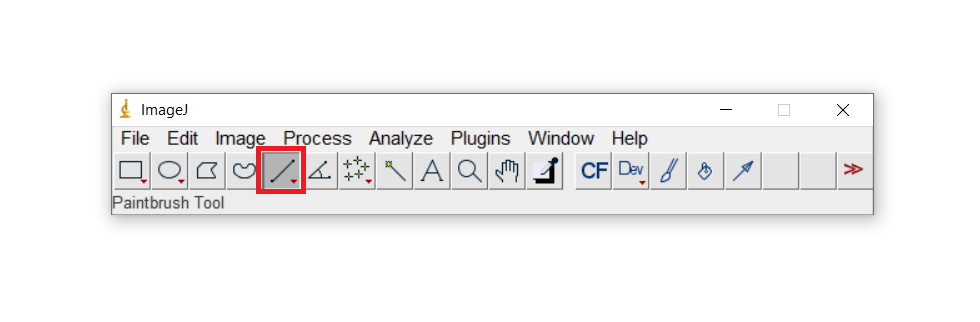
\includegraphics[width=0.7\textwidth]{galactic-center/line_tool.png}
	\caption {Top panel of ImageJ software with straight line tool highlighted}
	\label{gc:fig:linetool}
\end{figure}

\begin{figure}
	\centering
	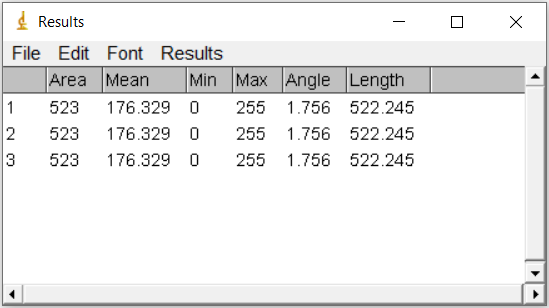
\includegraphics[width=0.7\textwidth]{galactic-center/measurement_table.png}
	\caption {Table generated by ImageJ when measuring}
	\label{gc:fig:measurement}
\end{figure}

\begin{steps}
	\item First, note the white arrow located on the left-hand side of the image. This indicates the angular scale of the image. In the top menu bar, click on the straight line icon (see  figure \ref{gc:fig:linetool}). Now click one end of the arrow and drag the line to the other end.
	
	\item Normally, the straight line tool measures pixel count, however, you can change the scale so that it gives you the the actual measurements according to the scale of the image. To do this, click on ``Analyze'' above the icons and select the ``set scale'' option. In the ``known distance'' box enter 0.1. This allows you to measure the angular separation \textit{d} of the objects in the image in arcseconds. 
	
	\item Once the scale is set, use the straight line tool (the same you used to set the scale) and draw a line from Sag A* to an orbiting star and hit ``m'' on the keyboard. This will generate a window with different measurements which updates each time you hit ``m'' (see figure \ref{gc:fig:measurement} for an example table). You will only be using the ``length'' (in arcseconds) and ``angle'' (in degrees) measurements. 
	\begin{framed}
		As stated, for this lab you will be focusing on the ``angular separation'' $d$ in arcseconds as well as the ``angle'' which gives the angular orientation of the line in degrees. This might seem confusing as in one instance you are using an angle measurement as a distance and in the other you are using it in a more familiar manner. This measurement quirk stems from how we measure distant astronomical objects. However, in order to avoid confusion, just remember that if a formula or asks for $\theta$ it is asking for the angular orientation of the object in the image and if it asks for $d$ it is asking for the distance measurement in arcseconds. 
	\end{framed}
\end{steps}

\subsubsection{Measuring data for S0-2 and S0-37}
Now you are ready to begin gathering data from the video. However, there are many different objects which you could measure and in order to avoid confusion you will be measuring two stars near Sag A* labeled S0-2 and S0-37 respectively. Using the data from these two stars and Kepler's laws, you will be able to calculate an approximate mass and size for Sag A*.  

\begin{table}
	\centering
	\begin{tabular}{c|c|c|c|c|c}
		frame & $d$ (arcseconds) & $s$ (cm) & $\theta$ (radians) & $\Delta \theta$ (radians) & $A$ (cm$^2$)
		\\ \midrule
		1 & & & & \cellcolor{black!25} & \cellcolor{black!25}
		\\ \midrule
		2 & & & & & 
		\\ \midrule
		3 & & & &  &
		\\ \midrule
		4 & & & &  &
		\\ \midrule
		5 & & & & &
		\\ \midrule
		6 & & & & &
		\\ \midrule
		7 & & & & &
		\\ \midrule
		8 & & & & &
		\\ \midrule
		9 & & & & &
		\\ \bottomrule
	\end{tabular}
	\caption{Data table for one stellar orbit. Note that you will not have any calculations for the gray cells for frame 1, since there is no previous frame to compare to.}\label{gc:tab:orbits}
\end{table}		
\begin{steps}
	\item First, in your lab reports make two separate tables following the format from Table \ref{gc:tab:orbits}, one for each star you will track.
	
	\item Now, load the first frame in ImageJ and locate the stars labeled S0-2 and S0-37. Using the straight line tool, measure the angular separation $d$ from Sag A* to both stars, as well as the angle $\theta$.  \textbf{Record these measurements in the respective table for each star}
	
	\item Now convert the angular separation from arcseconds to radians, then multiply by $2.47 \pm 0.05 \times 10^{22}$cm. This gives you the actual distance $s$ in centimeters. \textbf{Record this in the table under the \textit{s} column}
	
	\item Afterwards, convert the angle $\theta$ from degrees to radians.
	
	\item After you have calculated the distance $s$ in cm and the angle $\theta$ in radians for all frames, calculate the area swept out the stars using
	\begin{equation}
		A_i = \pi \left( \frac{s_{i} + s_{i-1}}{2} \right)^2 \left( \frac{\theta_{i}-\theta_{i-1}}{2\pi} \right) \,,
	\end{equation}
	where \textit{i} and $i-1$ are a frame and the frame before it respectively. This equation gives the area by taking the average of the separation of the object from the central mass, then multiplying it by the fraction of circle covered between the two points. Find the area covered each frame (except for the first). \textbf{Record these in the table}
	
	\item Based on your measurements and calculations, does Kepler's second law hold? Are there any discrepancies? What factors could account for these discrepancies? \textbf{record your answers int the lab report}
	
	\item Now, starting from the beginning of the video, estimate the orbital period for both S0-2 and S0-37. Use the time-stamp in the top-left corner (YEAR/MONTH) and convert your estimate into seconds. \textit{Hint: S0-37 does not complete a full orbit. However, we know that its orbit is circular. Using this fact and accounting for the effects of inclination, estimate S0-37s period} \textbf{Record in your lab report}
	
	\item After estimating the orbital periods, for S0-2 and S0-37, use the equation from Kepler's third law to calculate the mass of Sag A*, using the final measurement for \textit{s} as the value for \textit{a}. How does this compare to the mass $M_\mathrm{bh} = 4.0 \times 10^6\:\textrm{M}_\textrm{\astrosun}$ as measured by Boehle \textit{et. al.} in 2016?
	
	\item How different was your estimate from the true mass? What factors could have contributed to this difference? What assumptions did you have to make when estimating the period? How did you account for the effects of inclination? Why can we use Kepler's third law here? \textbf{Write down your answers in the lab report}
	
	\item Now, using the last frame of the image, use the orbital path traced in the video which came closest to Sag A* to place an upper limit on its radius. Use the straight line tool to measure this limit in arcseconds and convert to cm the same way as before. 
	
	
\end{steps}
\section{General Relativity and Schwarzschild Radii}
While Newtonian dynamics is useful for describing most orbital systems, extreme systems or objects such as black holes cannot be fully described without also incorporating general relativity. In particular for this lab we will be using a particular description of the universe in which gravity, rather than being an ``attraction'' between objects, is actually the result of curved ``space-time''. To visualize this, imagine space-time as sheet of stretched out fabric. Normally, if you were to try to roll light objects across the sheet they would travel in a straight line. However, if you were to place a large weight in the center, the fabric would ``droop'' inwards and any object you tried to roll would instead fall inwards towards the depressed region (the following video demonstrates this analogy \url{https://youtu.be/MTY1Kje0yLg}). This is analogous to the effect that gravity has on spacetime. The key to this description is that anything traveling through spacetime will follow this curvature, even if it has no mass such as light. This means that, theoretically, an object can exist which bends spacetime so much that not even light can climb back out and escape. Luckily, using the principles of gravitation developed by Newton, we can estimate how massive and small such an object would be.

\subsection{Steps}
\begin{steps}
	\item In Newtonian dynamics, the minimum speed an object needs to escape the gravitational pull of an object is given by 
	\begin{equation}\label{gc:eq:escape-speed}
		v_\textrm{escape} = \sqrt{\frac{2 G M}{r}} \,.
	\end{equation}
	where $r$ is the distance from its center of mass $M$. First, manipulate this equation in order to get an expression for $r$ in terms of the other values.
	
	\item If you now plug in the speed of light $c = 2.998 \times 10^{10}$cm/s as the escape velocity into the equation you just derived, you get an expression for what is known as the Schwarszchild radius. The Schwarzschild radius is an estimate of the upper limit of the radius of a black hole with a given mass. That is, according to this model, if a chunk of matter of mass M is squeezed into a radius as small or smaller than the radius $r$, then light cannot escape, and it behaves as a black hole. 
	\begin{enumerate}
		\item One of your group members.
		\item the Earth.
		\item the Sun.
		\item the Solar System.
		\item The Milky Way Galaxy.
	\end{enumerate}
	
	\item Now, using the estimate you found for the mass of Sag A*, calculate its Schwarzschild radius. How does this compare to the upper limit you estimated for its radius? 
	
	\item Based on this alone, how likely do you think it is that Sag A* is a black hole? What additional evidence would you need in order to conclude this? What sources of error could be affecting your estimates? 
	
	\item Go back and watch the video you watched at the start of the lab. This time, focus on one or two orbits and not how they change as the camera moves. How does the observed 2D shape of the orbit change? \textbf{Record your observations in the lab report}
	
	\item Once you have a good idea of how the change in perspective affects our observation of the different orbits, discuss in your groups what how this might lead to errors when estimating orbital parameters. Think back to the different calculations you made throughout the lab, what errors could have arisen from assuming that you were always observing orbits directly from above? If we tried using this assumption to calculate the mass of the central object in an orbit, will the mass be over or under-estimated? \textbf{Record your response in the lab report}
\end{steps}

\section{Individual Homework}
Throughout the lab, you attempted to determine whether the object located at Sag A* was a black hole by constraining its size and mass through its gravitational influence on nearby stars. It is possible to place further constraints on its size by measuring the time between fluctuations in the electromagnetic signal emitted by the object. Although Sag A* does not emit any significant light in the optical range of the spectrum, it does emit strong X-ray and radio frequencies. Moreover, the signals in these frequencies flare up on average once a day for short periods of time. However, since the speed of light is finite, light from one side of the object facing away from us will take more time to reach us than light from the side facing us. We can take advantage of this time difference to estimate how big an object is. Use figure \ref{gc:fig:light-curve} to find an upper bound on the size of Sag A* in this way. How does this compare to the size you calculated during lab? 


\begin{figure}
	\centering
	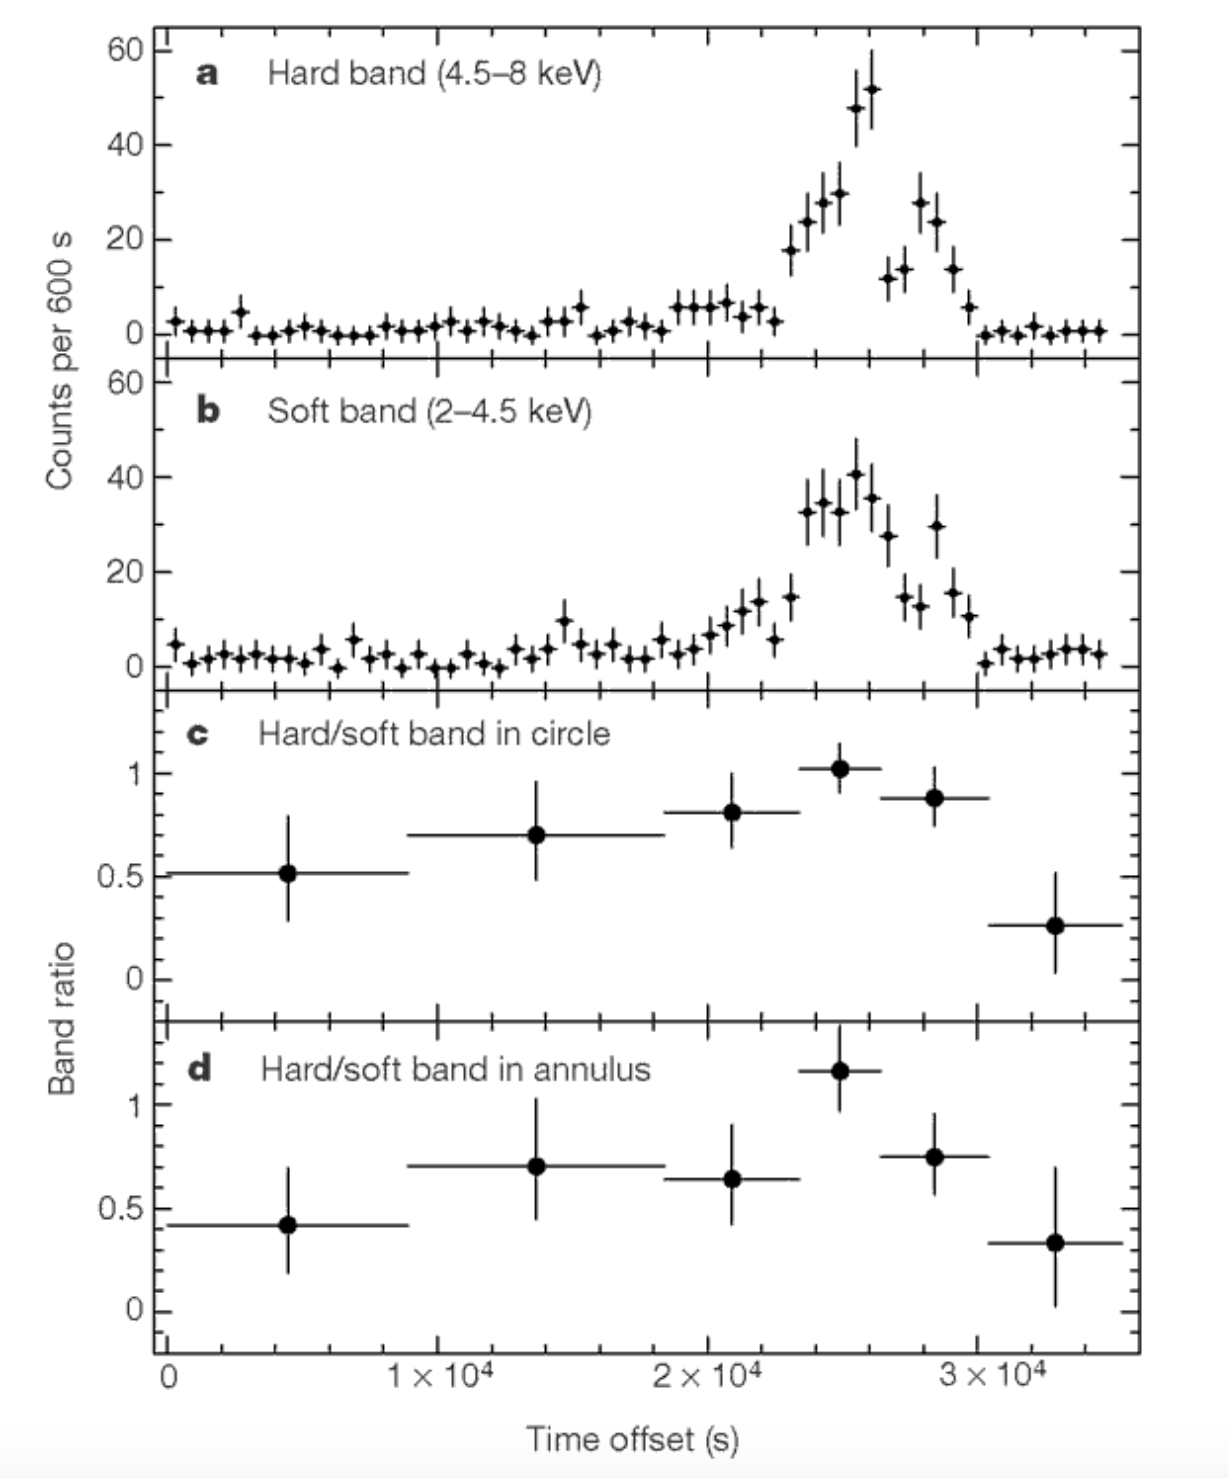
\includegraphics[width=0.7\textwidth]{galactic-center/sag-a-light-curve.png}
	\caption{Sag A* light curve, showing significant flaring on the timescale of a day.
		(from \url{https://heasarc.gsfc.nasa.gov/docs/objects/galaxies/sag-a star.html})}\label{gc:fig:light-curve}
\end{figure}


\appendix

\chapter{Analysis of Uncertainty}

A physical quantity consists of a value, unit, and uncertainty.
For example, ``$5 \pm 1\,$m'' means that the writer believes the true value of the quantity to most likely lie within 4 and 6 meters\footnote{The phrase ``most likely'' can mean different things depending on who is writing.
	If a physicist gives the value and does not given a further explanation, we can assume that they mean that the measurements are randomly distributed according to a normal distribution around the value given, with a standard deviation of the uncertainty given.
	So if one were to make the same measurement again, the author believes it has a 68\% chance of falling within the range given.
	Disciplines other than physics may intend the uncertainty to be 2 standard deviations.}.
Without knowing the uncertainty of a value, the quantity is next to useless.
For example, in our daily lives, we use an implied uncertainty.
If I say that we should meet at around 5:00 pm, and I arrive at 5:05 pm, you will probably consider that within the range that you would expect.
Perhaps your implied uncertainty is plus or minus 15 minutes.
On the other hand, if I said that we would meet at 5:07 pm, then if I arrive at 5:10 pm, you might be confused, since the implied uncertainty of that time value is more like 1 minute.

Scientists use the mathematics of probability and statistics, along with some intuition, to be precise and clear when talking about uncertainty, and it is vital to understand and report the uncertainty of quantitative results that we present.

\section{Types of measurement uncertainty}

For simplicity, we limit ourselves to the consideration of two types of uncertainty in this lab course, instrumental and random uncertainty.

\subsection{Instrumental uncertainties}

Every measuring instrument has an inherent uncertainty that is determined by the precision	
  of the instrument.
Usually this value is taken as a half of the smallest increment of the instrument's scale. For example, $0.5\:$mm is the precision of a standard metric ruler; $0.5\:$s is the precision of a watch, etc. For electronic digital displays, the equipment's manual often gives the instrument's resolution, which may be larger than that given by the rule above.

Instrumental uncertainties are the easiest ones to estimate, but they are not the only source of the uncertainty in your measured value.
You must be a skillful experimentalist to get rid of all other sources of uncertainty so that all that is left is instrumental uncertainty.

\subsection{Random uncertainties}

Very often when you measure the same physical quantity multiple times, you can get different results each time you measure it.
That happens because different uncontrollable factors affect your results randomly.
This type of uncertainty, random uncertainty, can be estimated only by repeating the same measurement several times.
For example if you measure the distance from a cannon to the place where the fired cannonball hits the ground, you could get different distances every time you repeat the same experiment.	
  
For example, say you took three measurements and obtained 55.7, 49.0, 52.5, 42.4, and 60.2 meters. We can quantify the variation in these measurements by finding their standard deviation using a calculator, spreadsheet, or the formula (assuming the data distributed according to a normal distribution)
\begin{equation}
 \sigma = \sqrt{\sum_{i=1}^{N} \frac{(x_i-\bar{x})^2}{N-1}} \, ,
\end{equation}
where $\{x_1, x_2, \dots, x_N\}$ are the measured values, $\bar{x}$ is the mean of those values, and $N$ is the number of measurements.
For our example, the resulting standard deviation is 6.8 meters. Generally we are interested not in the variation of the measurements themselves, but how uncertain we are of the average of the measurements. The uncertainty of this mean value is given, for a normal distribution, by the so-called ``standard deviation of the mean'', which can be found by dividing the standard deviation by the square root of the number of measurements,
\begin{equation}
\sigma_\textrm{mean} = \frac{\sigma}{\sqrt{N}} \, .
\end{equation}
So, in this example, the uncertainty of the mean is 3.0 meters. We can thus report the length as $52 \pm 3\:$m.

Note that if we take more measurements, the standard deviation of those measurements will not generally change, since the variability of our measurements shouldn't change over time. However, the standard deviation of the mean, and thus the uncertainty, will decrease.

\section{Propagation of uncertainty}

When we use an uncertain quantity in a calculation, the result is also uncertain. To determine by how much, we give some simple rules for basic calculations, and then a more general rule for use with any calculation which requires knowledge of calculus. Note that these rules are strictly valid only for values that are normally distributed, though for the purpose of this course, we will use these formulas regardless of the underlying distributions, unless otherwise stated, for simplicity.

If the measurements are completely independent of each other, then for quantities $a \pm \delta a$ and $b \pm \delta b$, we can use the following formulas:
\begin{equation}\label{unc:add}
\textrm{For } c = a + b \textrm{ (or for subtraction), } \delta c = \sqrt{(\delta a)^2 + (\delta b)^2}
\end{equation}

\begin{equation}\label{unc:mult}
\textrm{For } c = ab \textrm{ (or for division), } \frac{\delta c}{c} = \sqrt{\left(\frac{\delta a}{a}\right)^2 + \left(\frac{\delta b}{b}\right)^2}
\end{equation}

\begin{equation}\label{unc:exp}
\textrm{For } c = a^n,\, \frac{\delta c}{c} = n \frac{\delta a}{a}
\end{equation}

If you are familiar with calculus, you may want to use this general formula for the uncertainty $\delta f$ of a function $f$ of $N$ independent values $x_i$, each with uncertainty $\delta x_i$:
\begin{equation}\label{unc:general}
\delta f = \sqrt{ \sum_{i=1}^{N} \left(\frac{\partial f}{\partial x_i} \delta x_i\right)^2 } \, .
\end{equation}
Notice that Eqs.\ \ref{unc:add} through \ref{unc:exp} can be derived from Eq.\ \ref{unc:general} for those specific cases.

\subsubsection{What if there is no reported uncertainty?}

Sometimes you'll be calculating with numbers that have no uncertainty given.
In some cases, the number is exact.
For example, the circumference $C$ of a circle is given by $C = 2 \pi r$. Here, the coefficient, $2\pi$, is an exact quantity and you can treat its uncertainty as zero.
If you find a value that you think is uncertain, but the uncertainty is not given, a good rule of thumb is to assume that the uncertainty is half the right-most significant digit.
So if you are given a measured length of $1400\:$m, then you might assume that the uncertainty is $50\:$m.
This is an assumption, however, and should be described as such in your lab report.
For more examples, see Table~\ref{unc:tab:implied}.

\begin{table}
	\begin{center}
		\begin{tabular}{cc}
			\textbf{Expression} & \textbf{Implied uncertainty} \\
			12 & 0.5 \\
			12.0 & 0.05 \\
			120 & 5 \\
			120. & 0.5
		\end{tabular}
		\caption{Expression of numbers and their implied uncertainty.}\label{unc:tab:implied}
	\end{center}
\end{table}

\subsubsection{How many digits to report?}

After even a single calculation, a calculator will often give ten or more digits in an answer.
For example, if I travel $11.3 \pm 0.1\:$km in $350 \pm 10\:$s, then my average speed will be the distance divided by the duration. Entering this into my calculator, I get the resulting value ``\texttt{0.0322857142857143}''.
Perhaps it is obvious that my distance and duration measurements were not precise enough for all of those digits to be useful information.
We can use the propagated uncertainty to decide how many decimals to include.
Using the formulas above, I find that the uncertainty in the speed is given by my calculator as ``\texttt{9.65683578099600e-04}'', where the `\texttt{e}' stands for ``times ten to the''.
I definitely do not know my uncertainty to 14 decimal places.
For reporting uncertainties, it general suffices to use just the 1 or 2 left-most significant digits, unless you have a more sophisticated method of quantifying your uncertainties.
So here, I would round this to 1 significant digit, resulting in an uncertainty of $0.001\:$km/s.
Now I have a guide for how many digits to report in my value.
Any decimal places to the right of the one given in the uncertainty are distinctly unhelpful, so I report my average speed as ``$0.032 \pm 0.001\:$km/s''.
You may also see the equivalent, more succinct notation ``$0.032(1)\:$km/s''.

\section{Comparing two values}\label{unc:sec:comparing}

If we compare two quantities and want to find out how different they are from each other, we can use a measure we call a $t'$ value (pronounced ``tee prime''). This measure is not a standard statistical measure, but it is simple and its meaning is clear for us.

Operationally, for two quantities having the same unit, $a \pm \delta a$ and $b \pm \delta b$, the measure is defined as\footnote{Statistically, if $\delta a$ and $\delta b$ are uncorrelated, random uncertainties, then $t'$ represents how many standard deviations the difference $a - b$ is away from zero.}

\begin{equation}
%t' = \frac{\abs{a-b}}{\sqrt{(\delta a)^2 + (\delta b)^2}}
t' = \frac{\abs{a-b}}{\sqrt{(\delta a)^2 + (\delta b)^2}}
\end{equation}

If $t' \lesssim 1$, then the values are so close to each other that they are indistinguishable. It is either that they represent the same true value, or that the measurement should be improved to reduce the uncertainty.

If $1 \lesssim t' \lesssim 3$, then the result is inconclusive. One should improve the experiment to reduce the uncertainty.

If $t' \gtrsim 3$, then the true values are very probably different from each other.
\begin{landscape}
\chapter{Rubrics}
	
	\freetabcaption{Rubric B: Ability to design and conduct an observational experiment \cite{etkina_scientific_2006}.}
	\begin{longtable}{>{\bfseries}p{0.02\textheight}|>{\bfseries\RaggedRight}p{0.25\textheight}|>{\RaggedRight}p{0.21\textheight}|>{\RaggedRight}p{0.21\textheight}|>{\RaggedRight}p{0.22\textheight}|>{\RaggedRight}p{0.22\textheight}}
		\toprule
		& Scientific Ability
		& Missing & Inadequate & Needs Improvement & Adequate \\ \midrule \endhead
		B1
		& Is able to identify the phenomenon to be investigated
		& No phenomenon is mentioned
		& The description of the phenomenon to be investigated is confusing, or it is not the phenomenon of interest.
		& \midsloppy The description of the phenomenon is vague or incomplete.
		& The phenomenon to be investigated is clearly stated. \\ \midrule
		B2
		& Is able to design a reliable experiment that investigates the phenomenon
		& The experiment does not investigate the phenomenon.
		& The experiment may not yield any interesting patterns.
		& Some important aspects of the phenomenon will not be observable.
		& The experiment might yield interesting patterns relevant to the investigation of the phenomenon. \\ \midrule
		B3
		& Is able to decide what physical quantities are to be measured and identify independent and dependent variables
		& The physical quantities are irrelevant.
		& Only some of physical quantities are relevant.
		& The physical quantities are relevant. However, independent and dependent variables are not identified.
		& The physical quantities are relevant and independent and dependent variables are identified. \\ \midrule
		B4
		& Is able to describe how to use available equipment to make measurements
		& At least one of the chosen measurements cannot be made with the available equipment.
		& All chosen measurements can be made, but no details are given about how it is done.
		& All chosen measurements can be made, but the details of how it is done are vague or incomplete.
		& All chosen measurements can be made and all details of how it is done are clearly provided. \\ \midrule
		B5
		& Is able to describe what is observed without trying to explain, both in words and by means of a picture of the experimental setup.
		& No description is mentioned.
		& A description is incomplete. No labeled sketch is present. Or, observations are adjusted to fit expectations.
		& A description is complete, but mixed up with explanations or pattern. Or the sketch is present but is difficult to understand.
		& Clearly describes what happens in the experiments both verbally and with a sketch. Provides other representations when necessary (tables and graphs). \\ \midrule
		B6
		& Is able to identify the shortcomings in an experiment and suggest improvements
		& No attempt is made to identify any shortcomings of the experiment.
		& The shortcomings are described vaguely and no suggestions for improvement are made.
		& Not all aspects of the design are considered in terms of shortcomings or improvements.
		& All major shortcomings of the experiment are identified and reasonable suggestions for improvement are made. \\ \midrule
		B7
		& Is able to identify a pattern in the data
		& No attempt is made to search for a pattern.
		& The pattern described is irrelevant or inconsistent with the data.
		& The pattern has minor errors or omissions. Terms like ``proportional'' used without clarity, e.g.\ is the proportionality linear, quadratic, etc.
		& The pattern represents the relevant trend in the data. When possible, the trend is described in words. \\ \midrule
		B8
		& Is able to represent a pattern mathematically (if applicable)
		& No attempt is made to represent a pattern mathematically.
		& The mathematical expression does not represent the trend.
		& No analysis of how well the expression agrees with the data is included, or some features of the pattern are missing.
		& The expression represents the trend completely and an analysis of how well it agrees with the data is included. \\ \midrule
		B9
		& Is able to devise an explanation for an observed pattern
		& No attempt is made to explain the observed pattern.
		& An explanation is vague, not testable, or contradicts the pattern.
		& An explanation contradicts previous knowledge or the reasoning is flawed.
		& A reasonable explanation is made. It is testable and it explains the observed pattern. \\
		\bottomrule
	\end{longtable}

	
%\end{table}

\end{landscape}
\chapter{Lab Report Format}

Following the last session of a particular lab, each person will be responsible for turning in a lab report. In a general sense, the labs should demonstrate Rubric Rows F1 and F2 (see Table~\ref{rubric:f}), in addition to the other rubric rows listed in the lab write-up.

\section{General}

\begin{itemize}
	\item The report should be typed for ease of reading. Text should be double-spaced, and the page margins (including headers and footers) should be approximately $2.5\:$cm, for ease of marking by the grader. Each page should be numbered.
	
	\item The first page should include the title of the lab; lab section day, time, and number; and the names of the other members of your lab team.
	
	\item If the rubric row refers to a particular part of your lab report, clearly label that part of the report with that rubric row. For example, you should label the section where you demonstrate uncertainty propagation with ``G2'' if that rubric row is being assessed in that lab.
\end{itemize}

\section{Organizing the report}

If the lab is clearly framed as an observational, testing, or application experiment, you can follow the corresponding rubric for the elements to include in the report (see, respectively, Rubrics B, C, and D in Appendix~\ref{cha:rubrics}).

In general, the report \textbf{must} include the following sections:
\begin{enumerate}
	\item \textbf{Introduction.} A written description of what the lab is designed to investigate and a brief summary of the procedure used. This section should be at least a full paragraph long, and not more than 3 double-space pages.
	
	You don't need to include too much detail here, but it should be a complete and concise description of the purpose and general method used in the lab. Imagine a classmate who hasn't seen the lab writeup asked you, ``what is this lab about? What do you do?'' You should be able to hand them your introduction, and they'd be able to understand the purpose and general structure of the lab. But you need not mention every step and calculation here.
	
	\item \textbf{Analysis and discussion.} For most labs that have more than one part, this should be broken up into parts and labeled in order. This section must include all of the following, in the same order in which these elements appear in the lab instructions.
	\begin{itemize}
		\item Any data that you've collected: tables, figures, measured values, sketches. Whenever possible, include an estimate of the uncertainty of measured values.
		
		\item Any calculations that you perform using your data, and the final results of your calculation. Note that you must show your work in order to demonstrate to the grader that you have actually done it. Even if you're just plugging numbers into an equation, you should write down the equation and all the values that go into it. This includes calculating uncertainty and propagation of uncertainty.
		
		\item If you are using software to perform a calculation, you should explicitly record what you've done. For example, ``Using Excel we fit a straight line to the velocity vs. time graph. The resulting equation is $v = (0.92\:\mathrm{m/s^2}) t + 0.2\:\mathrm{m/s}$.
		
		\item Answers to any questions that appear in the lab handout.
	\end{itemize}

	\item \textbf{Conclusion.} This can be very short, and will generally only require one or two paragraphs. In your conclusion, you should summarize the point of the lab and what you learned, both in the frame of a scientist conducting the experiment (``What did the experiment tell us about the world?'') and in the frame of a student (``What skills or mindsets did I learn?'').
\end{enumerate}

\section{Graphs, Tables, and Figures}

Any graph, table, or figure (a figure is any graphic, for example a sketch) should include a caption describing what it is about and what features are important, or any helpful orientation to it. The reader should be able to understand the basics of what a graph, table, or figure is saying and why it is important without referring to the text. For more examples, see any such element in this lab manual.

Each of these elements has some particular conventions.

\subsection{Tables}

A table is a way to represent tabular data in a quantitative, precise form. Each column in the table should have a heading that describes the quantity name and the unit abbreviation in parentheses. For example, if you are reporting distance in parsecs, then the column heading should be something like ``distance (pc)''. This way, when reporting the distance itself in the column, you do not need to list the unit with every number.

\subsection{Graphs}

A graph is a visual way of representing data. It is helpful for communicating a visual summary of the data and any patterns that are found.

The following are necessary elements of a graph of two-dimensional data (for example, distance vs. time, or current vs. voltage) presented in a scatter plot.

\begin{itemize}
	\item \textbf{Proper axes.} The conventional way of reading a graph is to see how the variable on the vertical axis changes when the variable on the horizontal axis changes. If there are independent and dependent variables, then the independent variable should be along the horizontal axis.
	
	\item \textbf{Axis labels.} The axes should each be labeled with the quantity name and the unit abbreviation in parentheses. For example, if you are plotting distance in parsecs, then the axis label should be something like ``distance (pc)''.
	
	\item \textbf{Uncertainty bars.} If any quantities have an uncertainty, then these should be represented with so-called ``error bars'', along both axes if present. If the uncertainties are smaller than the symbol used for the data points, then this should be explained in the caption.

\end{itemize}

%\chapter{Equipment Manual: PASCO Interferometer}

On the following pages is the manual for the PASCO Interferometer.

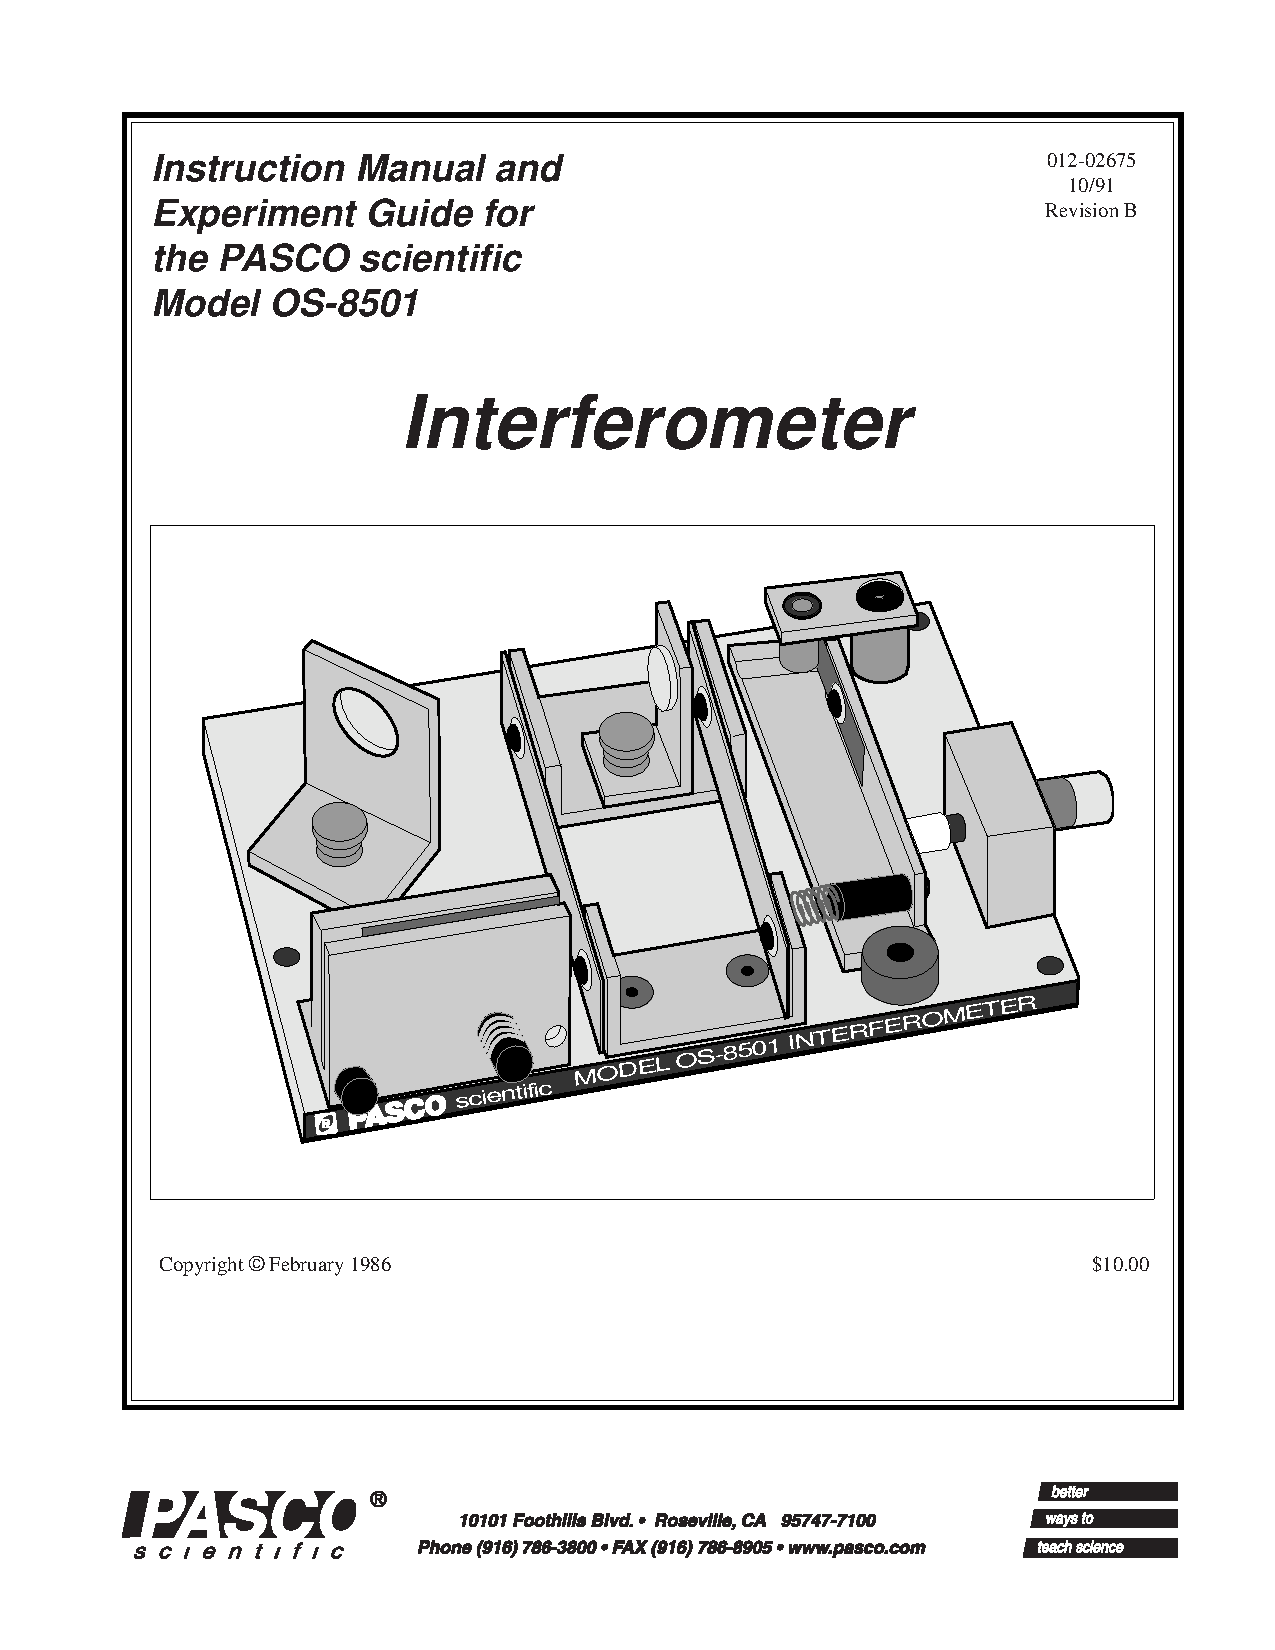
\includepdf[pages={1,6-8}]{pasco-interferometer/Introductory-Michelson-Interferometer-Manual-OS-8501.pdf}

\includepdf[pages={9-10}]{pasco-interferometer/Introductory-Michelson-Interferometer-Manual-OS-8501.pdf}
%\chapter{Manual: PASCO Cavendish Balance}\label{cha:pasco-cavendish}

On the following pages is the manual for the PASCO Cavendish Balance.

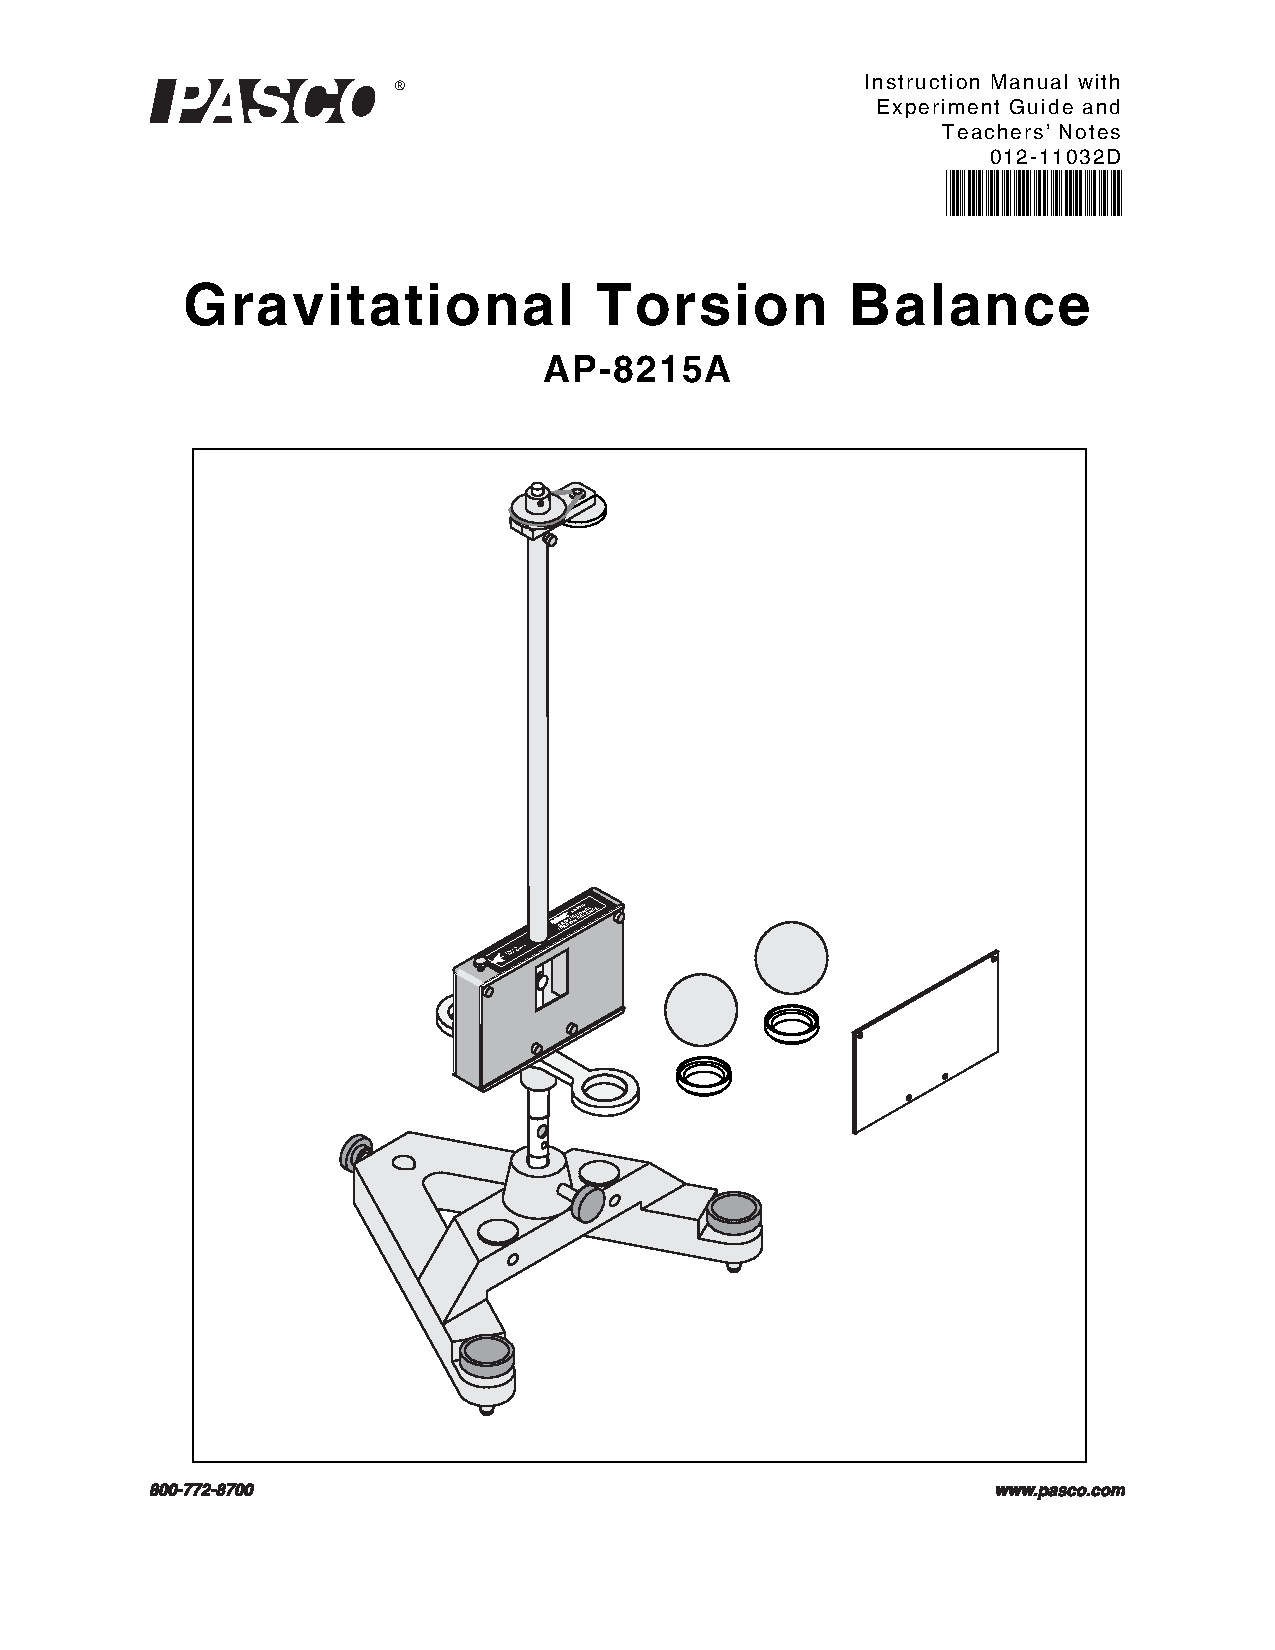
\includepdf[pages={1,3-8,16}]{pasco-cavendish/Gravitational-Torsion-Balance-Manual-AP-8215A.pdf}

% \bibliography{references,MyLibrary}
% \bibliographystyle{plain}
\printbibliography

\end{document}
